
%% bare_jrnl_compsoc.tex
%% V1.4b
%% 2015/08/26
%% by Michael Shell
%% See:
%% http://www.michaelshell.org/
%% for current contact information.
%%
%% This is a skeleton file demonstrating the use of IEEEtran.cls
%% (requires IEEEtran.cls version 1.8b or later) with an IEEE
%% Computer Society journal paper.
%%
%% Support sites:
%% http://www.michaelshell.org/tex/ieeetran/
%% http://www.ctan.org/pkg/ieeetran
%% and
%% http://www.ieee.org/

%%*************************************************************************
%% Legal Notice:
%% This code is offered as-is without any warranty either expressed or
%% implied; without even the implied warranty of MERCHANTABILITY or
%% FITNESS FOR A PARTICULAR PURPOSE! 
%% User assumes all risk.
%% In no event shall the IEEE or any contributor to this code be liable for
%% any damages or losses, including, but not limited to, incidental,
%% consequential, or any other damages, resulting from the use or misuse
%% of any information contained here.
%%
%% All comments are the opinions of their respective authors and are not
%% necessarily endorsed by the IEEE.
%%
%% This work is distributed under the LaTeX Project Public License (LPPL)
%% ( http://www.latex-project.org/ ) version 1.3, and may be freely used,
%% distributed and modified. A copy of the LPPL, version 1.3, is included
%% in the base LaTeX documentation of all distributions of LaTeX released
%% 2003/12/01 or later.
%% Retain all contribution notices and credits.
%% ** Modified files should be clearly indicated as such, including  **
%% ** renaming them and changing author support contact information. **
%%*************************************************************************


% *** Authors should verify (and, if needed, correct) their LaTeX system  ***
% *** with the testflow diagnostic prior to trusting their LaTeX platform ***
% *** with production work. The IEEE's font choices and paper sizes can   ***
% *** trigger bugs that do not appear when using other class files.       ***                          ***
% The testflow support page is at:
% http://www.michaelshell.org/tex/testflow/


\documentclass[10pt,journal,compsoc]{IEEEtran}
%
% If IEEEtran.cls has not been installed into the LaTeX system files,
% manually specify the path to it like:
% \documentclass[10pt,journal,compsoc]{../sty/IEEEtran}





% Some very useful LaTeX packages include:
% (uncomment the ones you want to load)


% *** MISC UTILITY PACKAGES ***
%
%\usepackage{ifpdf}
% Heiko Oberdiek's ifpdf.sty is very useful if you need conditional
% compilation based on whether the output is pdf or dvi.
% usage:
% \ifpdf
%   % pdf code
% \else
%   % dvi code
% \fi
% The latest version of ifpdf.sty can be obtained from:
% http://www.ctan.org/pkg/ifpdf
% Also, note that IEEEtran.cls V1.7 and later provides a builtin
% \ifCLASSINFOpdf conditional that works the same way.
% When switching from latex to pdflatex and vice-versa, the compiler may
% have to be run twice to clear warning/error messages.






% *** CITATION PACKAGES ***
%
\ifCLASSOPTIONcompsoc
  % IEEE Computer Society needs nocompress option
  % requires cite.sty v4.0 or later (November 2003)
  \usepackage[nocompress]{cite}
\else
  % normal IEEE
  \usepackage{cite}
\fi
% cite.sty was written by Donald Arseneau
% V1.6 and later of IEEEtran pre-defines the format of the cite.sty package
% \cite{} output to follow that of the IEEE. Loading the cite package will
% result in citation numbers being automatically sorted and properly
% "compressed/ranged". e.g., [1], [9], [2], [7], [5], [6] without using
% cite.sty will become [1], [2], [5]--[7], [9] using cite.sty. cite.sty's
% \cite will automatically add leading space, if needed. Use cite.sty's
% noadjust option (cite.sty V3.8 and later) if you want to turn this off
% such as if a citation ever needs to be enclosed in parenthesis.
% cite.sty is already installed on most LaTeX systems. Be sure and use
% version 5.0 (2009-03-20) and later if using hyperref.sty.
% The latest version can be obtained at:
% http://www.ctan.org/pkg/cite
% The documentation is contained in the cite.sty file itself.
%
% Note that some packages require special options to format as the Computer
% Society requires. In particular, Computer Society  papers do not use
% compressed citation ranges as is done in typical IEEE papers
% (e.g., [1]-[4]). Instead, they list every citation separately in order
% (e.g., [1], [2], [3], [4]). To get the latter we need to load the cite
% package with the nocompress option which is supported by cite.sty v4.0
% and later. Note also the use of a CLASSOPTION conditional provided by
% IEEEtran.cls V1.7 and later.





% *** GRAPHICS RELATED PACKAGES ***
%
\ifCLASSINFOpdf
  \usepackage[pdftex]{graphicx}
  \usepackage{subfigure}
  % declare the path(s) where your graphic files are
  % \graphicspath{{../pdf/}{../jpeg/}}
  % and their extensions so you won't have to specify these with
  % every instance of \includegraphics
  % \DeclareGraphicsExtensions{.pdf,.jpeg,.png}
\else
  % or other class option (dvipsone, dvipdf, if not using dvips). graphicx
  % will default to the driver specified in the system graphics.cfg if no
  % driver is specified.
  % \usepackage[dvips]{graphicx}
  % declare the path(s) where your graphic files are
  % \graphicspath{{../eps/}}
  % and their extensions so you won't have to specify these with
  % every instance of \includegraphics
  % \DeclareGraphicsExtensions{.eps}
\fi
% graphicx was written by David Carlisle and Sebastian Rahtz. It is
% required if you want graphics, photos, etc. graphicx.sty is already
% installed on most LaTeX systems. The latest version and documentation
% can be obtained at: 
% http://www.ctan.org/pkg/graphicx
% Another good source of documentation is "Using Imported Graphics in
% LaTeX2e" by Keith Reckdahl which can be found at:
% http://www.ctan.org/pkg/epslatex
%
% latex, and pdflatex in dvi mode, support graphics in encapsulated
% postscript (.eps) format. pdflatex in pdf mode supports graphics
% in .pdf, .jpeg, .png and .mps (metapost) formats. Users should ensure
% that all non-photo figures use a vector format (.eps, .pdf, .mps) and
% not a bitmapped formats (.jpeg, .png). The IEEE frowns on bitmapped formats
% which can result in "jaggedy"/blurry rendering of lines and letters as
% well as large increases in file sizes.
%
% You can find documentation about the pdfTeX application at:
% http://www.tug.org/applications/pdftex






% *** MATH PACKAGES ***
%
\usepackage{amsmath}
\usepackage{amsthm}
% A popular package from the American Mathematical Society that provides
% many useful and powerful commands for dealing with mathematics.
%
% Note that the amsmath package sets \interdisplaylinepenalty to 10000
% thus preventing page breaks from occurring within multiline equations. Use:
%\interdisplaylinepenalty=2500
% after loading amsmath to restore such page breaks as IEEEtran.cls normally
% does. amsmath.sty is already installed on most LaTeX systems. The latest
% version and documentation can be obtained at:
% http://www.ctan.org/pkg/amsmath





% *** SPECIALIZED LIST PACKAGES ***
%
\usepackage{algorithm}
\usepackage{algorithmic}
% algorithmic.sty was written by Peter Williams and Rogerio Brito.
% This package provides an algorithmic environment fo describing algorithms.
% You can use the algorithmic environment in-text or within a figure
% environment to provide for a floating algorithm. Do NOT use the algorithm
% floating environment provided by algorithm.sty (by the same authors) or
% algorithm2e.sty (by Christophe Fiorio) as the IEEE does not use dedicated
% algorithm float types and packages that provide these will not provide
% correct IEEE style captions. The latest version and documentation of
% algorithmic.sty can be obtained at:
% http://www.ctan.org/pkg/algorithms
% Also of interest may be the (relatively newer and more customizable)
% algorithmicx.sty package by Szasz Janos:
% http://www.ctan.org/pkg/algorithmicx




% *** ALIGNMENT PACKAGES ***
%
%\usepackage{array}
% Frank Mittelbach's and David Carlisle's array.sty patches and improves
% the standard LaTeX2e array and tabular environments to provide better
% appearance and additional user controls. As the default LaTeX2e table
% generation code is lacking to the point of almost being broken with
% respect to the quality of the end results, all users are strongly
% advised to use an enhanced (at the very least that provided by array.sty)
% set of table tools. array.sty is already installed on most systems. The
% latest version and documentation can be obtained at:
% http://www.ctan.org/pkg/array


% IEEEtran contains the IEEEeqnarray family of commands that can be used to
% generate multiline equations as well as matrices, tables, etc., of high
% quality.




% *** SUBFIGURE PACKAGES ***
%\ifCLASSOPTIONcompsoc
%  \usepackage[caption=false,font=footnotesize,labelfont=sf,textfont=sf]{subfig}
%\else
%  \usepackage[caption=false,font=footnotesize]{subfig}
%\fi
% subfig.sty, written by Steven Douglas Cochran, is the modern replacement
% for subfigure.sty, the latter of which is no longer maintained and is
% incompatible with some LaTeX packages including fixltx2e. However,
% subfig.sty requires and automatically loads Axel Sommerfeldt's caption.sty
% which will override IEEEtran.cls' handling of captions and this will result
% in non-IEEE style figure/table captions. To prevent this problem, be sure
% and invoke subfig.sty's "caption=false" package option (available since
% subfig.sty version 1.3, 2005/06/28) as this is will preserve IEEEtran.cls
% handling of captions.
% Note that the Computer Society format requires a sans serif font rather
% than the serif font used in traditional IEEE formatting and thus the need
% to invoke different subfig.sty package options depending on whether
% compsoc mode has been enabled.
%
% The latest version and documentation of subfig.sty can be obtained at:
% http://www.ctan.org/pkg/subfig




% *** FLOAT PACKAGES ***
%
%\usepackage{fixltx2e}
% fixltx2e, the successor to the earlier fix2col.sty, was written by
% Frank Mittelbach and David Carlisle. This package corrects a few problems
% in the LaTeX2e kernel, the most notable of which is that in current
% LaTeX2e releases, the ordering of single and double column floats is not
% guaranteed to be preserved. Thus, an unpatched LaTeX2e can allow a
% single column figure to be placed prior to an earlier double column
% figure.
% Be aware that LaTeX2e kernels dated 2015 and later have fixltx2e.sty's
% corrections already built into the system in which case a warning will
% be issued if an attempt is made to load fixltx2e.sty as it is no longer
% needed.
% The latest version and documentation can be found at:
% http://www.ctan.org/pkg/fixltx2e


%\usepackage{stfloats}
% stfloats.sty was written by Sigitas Tolusis. This package gives LaTeX2e
% the ability to do double column floats at the bottom of the page as well
% as the top. (e.g., "\begin{figure*}[!b]" is not normally possible in
% LaTeX2e). It also provides a command:
%\fnbelowfloat
% to enable the placement of footnotes below bottom floats (the standard
% LaTeX2e kernel puts them above bottom floats). This is an invasive package
% which rewrites many portions of the LaTeX2e float routines. It may not work
% with other packages that modify the LaTeX2e float routines. The latest
% version and documentation can be obtained at:
% http://www.ctan.org/pkg/stfloats
% Do not use the stfloats baselinefloat ability as the IEEE does not allow
% \baselineskip to stretch. Authors submitting work to the IEEE should note
% that the IEEE rarely uses double column equations and that authors should try
% to avoid such use. Do not be tempted to use the cuted.sty or midfloat.sty
% packages (also by Sigitas Tolusis) as the IEEE does not format its papers in
% such ways.
% Do not attempt to use stfloats with fixltx2e as they are incompatible.
% Instead, use Morten Hogholm'a dblfloatfix which combines the features
% of both fixltx2e and stfloats:
%
% \usepackage{dblfloatfix}
% The latest version can be found at:
% http://www.ctan.org/pkg/dblfloatfix




%\ifCLASSOPTIONcaptionsoff
%  \usepackage[nomarkers]{endfloat}
% \let\MYoriglatexcaption\caption
% \renewcommand{\caption}[2][\relax]{\MYoriglatexcaption[#2]{#2}}
%\fi
% endfloat.sty was written by James Darrell McCauley, Jeff Goldberg and 
% Axel Sommerfeldt. This package may be useful when used in conjunction with 
% IEEEtran.cls'  captionsoff option. Some IEEE journals/societies require that
% submissions have lists of figures/tables at the end of the paper and that
% figures/tables without any captions are placed on a page by themselves at
% the end of the document. If needed, the draftcls IEEEtran class option or
% \CLASSINPUTbaselinestretch interface can be used to increase the line
% spacing as well. Be sure and use the nomarkers option of endfloat to
% prevent endfloat from "marking" where the figures would have been placed
% in the text. The two hack lines of code above are a slight modification of
% that suggested by in the endfloat docs (section 8.4.1) to ensure that
% the full captions always appear in the list of figures/tables - even if
% the user used the short optional argument of \caption[]{}.
% IEEE papers do not typically make use of \caption[]'s optional argument,
% so this should not be an issue. A similar trick can be used to disable
% captions of packages such as subfig.sty that lack options to turn off
% the subcaptions:
% For subfig.sty:
% \let\MYorigsubfloat\subfloat
% \renewcommand{\subfloat}[2][\relax]{\MYorigsubfloat[]{#2}}
% However, the above trick will not work if both optional arguments of
% the \subfloat command are used. Furthermore, there needs to be a
% description of each subfigure *somewhere* and endfloat does not add
% subfigure captions to its list of figures. Thus, the best approach is to
% avoid the use of subfigure captions (many IEEE journals avoid them anyway)
% and instead reference/explain all the subfigures within the main caption.
% The latest version of endfloat.sty and its documentation can obtained at:
% http://www.ctan.org/pkg/endfloat
%
% The IEEEtran \ifCLASSOPTIONcaptionsoff conditional can also be used
% later in the document, say, to conditionally put the References on a 
% page by themselves.




% *** PDF, URL AND HYPERLINK PACKAGES ***
%
%\usepackage{url}
% url.sty was written by Donald Arseneau. It provides better support for
% handling and breaking URLs. url.sty is already installed on most LaTeX
% systems. The latest version and documentation can be obtained at:
% http://www.ctan.org/pkg/url
% Basically, \url{my_url_here}.

% Extra Packages
\usepackage{booktabs}
\usepackage{url}

% Extra Commands
\DeclareMathOperator*{\argmin}{arg\,min}


% *** Do not adjust lengths that control margins, column widths, etc. ***
% *** Do not use packages that alter fonts (such as pslatex).         ***
% There should be no need to do such things with IEEEtran.cls V1.6 and later.
% (Unless specifically asked to do so by the journal or conference you plan
% to submit to, of course. )


% correct bad hyphenation here
\hyphenation{op-tical net-works semi-conduc-tor}


\begin{document}
%
% paper title
% Titles are generally capitalized except for words such as a, an, and, as,
% at, but, by, for, in, nor, of, on, or, the, to and up, which are usually
% not capitalized unless they are the first or last word of the title.
% Linebreaks \\ can be used within to get better formatting as desired.
% Do not put math or special symbols in the title.
\title{Statistical Learning and Inference\\Project Report}
%
%
% author names and IEEE memberships
% note positions of commas and nonbreaking spaces ( ~ ) LaTeX will not break
% a structure at a ~ so this keeps an author's name from being broken across
% two lines.
% use \thanks{} to gain access to the first footnote area
% a separate \thanks must be used for each paragraph as LaTeX2e's \thanks
% was not built to handle multiple paragraphs
%
%
%\IEEEcompsocitemizethanks is a special \thanks that produces the bulleted
% lists the Computer Society journals use for "first footnote" author
% affiliations. Use \IEEEcompsocthanksitem which works much like \item
% for each affiliation group. When not in compsoc mode,
% \IEEEcompsocitemizethanks becomes like \thanks and
% \IEEEcompsocthanksitem becomes a line break with idention. This
% facilitates dual compilation, although admittedly the differences in the
% desired content of \author between the different types of papers makes a
% one-size-fits-all approach a daunting prospect. For instance, compsoc 
% journal papers have the author affiliations above the "Manuscript
% received ..."  text while in non-compsoc journals this is reversed. Sigh.

\author{Fuming~Zhang,~118033910025
\IEEEcompsocitemizethanks{
  \IEEEcompsocthanksitem Private leaderboard accuracy 0.93754 with rank 37
  \IEEEcompsocthanksitem Public leaderboard accuracy 0.94401 with rank 19
  \IEEEcompsocthanksitem E-mail: zhangfuming-alex@sjtu.edu.cn}}

% note the % following the last \IEEEmembership and also \thanks - 
% these prevent an unwanted space from occurring between the last author name
% and the end of the author line. i.e., if you had this:
% 
% \author{....lastname \thanks{...} \thanks{...} }
%                     ^------------^------------^----Do not want these spaces!
%
% a space would be appended to the last name and could cause every name on that
% line to be shifted left slightly. This is one of those "LaTeX things". For
% instance, "\textbf{A} \textbf{B}" will typeset as "A B" not "AB". To get
% "AB" then you have to do: "\textbf{A}\textbf{B}"
% \thanks is no different in this regard, so shield the last } of each \thanks
% that ends a line with a % and do not let a space in before the next \thanks.
% Spaces after \IEEEmembership other than the last one are OK (and needed) as
% you are supposed to have spaces between the names. For what it is worth,
% this is a minor point as most people would not even notice if the said evil
% space somehow managed to creep in.



% The paper headers
%\markboth{Journal of \LaTeX\ Class Files,~Vol.~14, No.~8, August~2015}%
%{Shell \MakeLowercase{\textit{et al.}}: Bare Demo of IEEEtran.cls for Computer Society Journals}
% The only time the second header will appear is for the odd numbered pages
% after the title page when using the twoside option.
% 
% *** Note that you probably will NOT want to include the author's ***
% *** name in the headers of peer review papers.                   ***
% You can use \ifCLASSOPTIONpeerreview for conditional compilation here if
% you desire.



% The publisher's ID mark at the bottom of the page is less important with
% Computer Society journal papers as those publications place the marks
% outside of the main text columns and, therefore, unlike regular IEEE
% journals, the available text space is not reduced by their presence.
% If you want to put a publisher's ID mark on the page you can do it like
% this:
%\IEEEpubid{0000--0000/00\$00.00~\copyright~2015 IEEE}
% or like this to get the Computer Society new two part style.
%\IEEEpubid{\makebox[\columnwidth]{\hfill 0000--0000/00/\$00.00~\copyright~2015 IEEE}%
%\hspace{\columnsep}\makebox[\columnwidth]{Published by the IEEE Computer Society\hfill}}
% Remember, if you use this you must call \IEEEpubidadjcol in the second
% column for its text to clear the IEEEpubid mark (Computer Society jorunal
% papers don't need this extra clearance.)



% use for special paper notices
%\IEEEspecialpapernotice{(Invited Paper)}



% for Computer Society papers, we must declare the abstract and index terms
% PRIOR to the title within the \IEEEtitleabstractindextext IEEEtran
% command as these need to go into the title area created by \maketitle.
% As a general rule, do not put math, special symbols or citations
% in the abstract or keywords.
\iffalse
\IEEEtitleabstractindextext{%
\begin{abstract}
  Abstract
\end{abstract}

% Note that keywords are not normally used for peerreview papers.
\begin{IEEEkeywords}
  Keywords
\end{IEEEkeywords}}
\fi


% make the title area
\maketitle


% To allow for easy dual compilation without having to reenter the
% abstract/keywords data, the \IEEEtitleabstractindextext text will
% not be used in maketitle, but will appear (i.e., to be "transported")
% here as \IEEEdisplaynontitleabstractindextext when the compsoc 
% or transmag modes are not selected <OR> if conference mode is selected 
% - because all conference papers position the abstract like regular
% papers do.
\IEEEdisplaynontitleabstractindextext
% \IEEEdisplaynontitleabstractindextext has no effect when using
% compsoc or transmag under a non-conference mode.



% For peer review papers, you can put extra information on the cover
% page as needed:
% \ifCLASSOPTIONpeerreview
% \begin{center} \bfseries EDICS Category: 3-BBND \end{center}
% \fi
%
% For peerreview papers, this IEEEtran command inserts a page break and
% creates the second title. It will be ignored for other modes.
\IEEEpeerreviewmaketitle



\IEEEraisesectionheading{\section{Introduction}\label{sec:introduction}}

In recent years, with the rapid development of deep learning, researchers have made significant progress in the fields of image recognition and natural language processing. Although deep neural networks can achieve better results in specific areas, their interpretability is still unsatisfactory. And the deeper the network, the harder it is to train and the more time it takes. Compared with the neural networks, the classical methods in statistical learning and inference are efficient and straightforward.

In this project, we are going to use some of the classical methods in statistical learning to solve the image classification problem under ImageNet. Although the principles of these methods are concise, it is quite complicated to implement from scratch. With the help of scikit-learn\cite{scikit-learn}, we can focus on the adjustment of the hyperparameters on the method and the comparison between different methods. We not only tried various classification methods such as ridge classification, logistic regression, linear discriminant analysis, support vector machine and k nearest neighbour classification, but also tried to perform data preprocessing and dimensionality reduction. After we augment the training set using a semi-supervised learning method, we selected the best model by k-fold cross-validation, we achieved an accuracy of 0.93754 on the test set and ranked 37th on the private leaderboard.

The remainder of this paper is organized as follows. In Section \ref{sec:data}, we describe the dataset this project and some related processing methods. Two dimensionality reduction methods are introduced in Section \ref{sec:dimensionality_reduction}. Then, the five classification methods we used is illustrated in Section \ref{sec:classification_methods}. We discuss the model selection approach in Section \ref{sec:model_selection}. Evaluation of all the above methods is described in Section \ref{sec:evaluation}. Finally, we conclude the paper in Section \ref{sec:conclusion}.


\section{Data}
\label{sec:data}
In this section, we will first provide a overview of the dataset in \ref{subsec:dataset_overview}, then we will introduce data preprocessing and augmentation in \ref{subsec:preprocessing} and \ref{subsec:augmentation}, respectively.

\subsection{Dataset Overview}
\label{subsec:dataset_overview}
In this project, data is collected from ImageNet, which contains 12 categories for classification. The dataset is split into training set and testing set. The training set contains 7800 images (650 images for each class), while the test set contains 15600 images (1300 images per class). The 4096 features provided are generated by a neural network trained on ImageNet.

By observing the training set, it is not difficult to find that each data has a value of 0 in many dimensions, and the values in all dimensions are greater than or equal to zero.

\subsection{Preprocessing}
\label{subsec:preprocessing}
Standardization of datasets is a common requirement for many machine learning estimators. Otherwise, they might behave badly if the individual features do not more or less look like standard normally distributed data: Gaussian with zero mean and unit variance. In practice we often ignore the shape of the distribution and just transform the data to center it by removing the mean value of each feature, then scale it by dividing non-constant features by their standard deviation.

For instance, many elements used in the objective function of a learning algorithm (such as the RBF kernel of Support Vector Machines or the l1 and l2 regularizers of linear models) assume that all features are centered around zero and have variance in the same order. If a feature has a variance that is orders of magnitude larger than others, it might dominate the objective function and make the estimator unable to learn from other features correctly as expected.

Therefore, we mainly use min-max scaling, l1 and l2 normalization these three preprocessing methods in this project. As for min-max scaling, we use the implementation provided by 'sklearn.preprocessing.MinMaxScaler' to scale the data to the $[0,1]$ interval. For l1 and l2 normalization, we use the implementation provided by 'sklearn.preprocessing.normalize'. By specifying the value of parameter 'norm' as 'l1' or 'l2', we scale input vectors individually to unit norm. The results of these preprocessing methods are compared in \ref{subsec:eva_ridge}.

\subsection{Augmentation}
\label{subsec:augmentation}

Limited by the number of training samples, after a series of hyperparameter and preprocessing adjustment model selection, our prediction accuracy is difficult to further improve, as if hit the accuracy wall. To solve this problem, we decide to add more data to the training set. There are many ways to augment existing datasets and produce more robust models. In the image domain, these are done to utilize the full power of the convolutional neural network, which is able to capture translational invariance. However, in this project, also limited by the number of samples, we have not tried to use the neural network method.

Considering that the given data is already in the form of generated features, we cannot perform transformations and color distortions to the data like images, but we can add some random noise to the data. However, we did not use the above method in practice. Instead, we choose the semi-supervised learning method which adds the same results predicted on the test set by several classifiers into the training set. By repeating this approach, we achieved the highest prediction accuracy of 93.754\% with ridge classifier on the private leaderboard.

\section{Dimensionality Reduction}
\label{sec:dimensionality_reduction}
In this section, we will introduce two dimensionality reduction methods, principle component analysis in \ref{subsec:pca} and factor analysis in \ref{subsec:fa}.

\subsection{Principle Component Analysis}
\label{subsec:pca}

Principle Component Analysis (abbreviation as PCA) is used to decompose a multivariate dataset in a set of successive orthogonal components that explain a maximum amount of the variance. Given a set of data in ${\rm IR}^p$, denote the observations by $x_1, x_2,...,x_N$, and consider the rank-$q$ linear model for representing them
\begin{equation}
  f(\lambda) = \mu + V_q\lambda,
\end{equation}
where $\mu$ is a location vector in ${\rm IR}^p$, $V_q$ is a $p \times q$ matrix with $q$ orthogonal unit vectors as columns, and $\lambda$ is a $q$ vector of parameters. Fitting such a model to the data by least squares amounts to minimizing the reconstruction error
\begin{equation}
  \min_{\mu, \{\lambda_i\}, V_q} \sum_{i=1}^N||x_i - \mu - V_q\lambda_i^2|.
\end{equation}

We can partially optimize for $\mu$ and the $\lambda_i$ to obtain
\begin{align}
  \hat{\mu} &= \bar{x},\\
  \hat{\lambda}_i &= V_q^T(x_i - \bar{x}).
\end{align}

This leaves us to find the orthogonal matrix $V_q$:
\begin{equation}
  \min_{V_q}\sum_{i=1}^N||(x_i - \bar{x}) - V_qV_q^T(x_i - \bar{x})||^2.
\end{equation}

The $p\times p$ matrix $H_q = V_qV_q^T$ is a projection matrix, and maps each point $x_i$ onto its rank-$q$ reconstruction $H_qx_i$, the orthogonal projection of $x_i$ onto the subspace spanned by the columns of $V_q$.

\subsection{Factor Analysis}
\label{subsec:fa}
The classical factor analysis model has the form
\begin{equation}
  X = AS + \epsilon.
\end{equation}

Here $S$ is a vector of $q < p$ underlying latent variables or factors, $A$ is a $p \times q$ matrix of factor loadings, and the $\epsilon_j$ are uncorrelated zero-mean disturbances. Typically the $S_l$ and the $\epsilon_j$ are modeled as Gaussian random variables, and the model is fit by maximum likelihood. The parameters all reside in the covariance matrix
\begin{equation}
  \Sigma = AA^T + D_{\epsilon},
\end{equation}
where $D_{\epsilon} = {\rm diag}[{\rm Var}(\epsilon_1),...,Var(\epsilon_p)]$. The columns of $A$ are referred to as the  factor loadings, and are used to name and interpret the factors.

Factor analysis can produce similar components (the columns of its loading matrix) to PCA. However, one can not make any general statements about these components. The main advantage for Factor Analysis over PCA is that it can model the variance in every direction of the input space independently (heteroscedastic noise). We followed the instructions given in \cite{pcavsfa} to find the best n\_components of our data set in this project and the results are shown in \ref{subsec:eva_pca}.

\section{Classification Methods}
\label{sec:classification_methods}
In this section, we will present the classification methods we used in this project. For each method, we first review its definition and basic principles, and then introduce how we use scikit-learn\cite{scikit-learn} based implementations.

\subsection{Ridge Regression}
\label{subsec:ridge_regression}
Compared with the ordinary least squares method, ridge regression shrinks the regression coefficients by imposing a penalty on their size. The ridge coefficients minimize a penalized residual sum of squares,
\begin{equation}
  \label{eq:ridge_regression}
  \hat{\beta}^{\rm ridge} = \argmin_{\beta}\left\{\sum_{i=1}^N(y_i - \beta_0 - \sum_{j=1}^px_{ij}\beta_j)^2 + \lambda\sum_{j=1}^p\beta_j^2\right\}.
\end{equation}

Here $\lambda \geq 0$ is a complexity parameter that controls the amount of shrinkage; the larger the value of $\lambda$, the greater the amount of shrinkage. The coefficients are shrunk toward zero (and each other)\cite{friedman2001elements}.

In this project, we use the implementation provided by 'sklearn.linear\_model.RidgeClassifier'. It is a classifier using ridge regression. When dealing with a multi-class classification task, n\_class classifiers are trained in a one-versus-all approach. Concretely, this is implemented by taking advantage of the multi-variate response support in ridge. Some important parameters of this method are introduced as follows:
\begin{itemize}
  \item \textbf{alpha}: It is a positive float indicating the regularization strength. Regularization improves the conditioning of the problem and reduces the variance of the estimates. Large values specify stronger regularization. It is worth noting that the alpha here corresponds to $C^{-1}$ in other linear models such as logistic regression and linear SVC.
  \item \textbf{normalize}: This is a boolean value which indicates whether to perform l2 normalization on the data. Its default value is false, and we have not used this parameter in our experiments. When we decide to perform data preprocessing, we will process the data before the model is trained.
  \item \textbf{class\_weight}: The value of this parameter should be a dictionary in Python or 'balanced', which denotes the weights associated with classes. If not given, all classes are supposed to have weight one. If 'balanced' mode is used, the weights are adjusted inversely proportional to class frequencies as $\frac{\rm n\_samples}{\rm n\_classes \times np.bincount(y)}$. Since the amount of data in each class is the same in our training set, the effect of using the 'balanced' mode and the default unspecified parameter is the same.
  \item \textbf{solver}: The candidate values for this parameter are 'auto', 'svd', 'cholesky', 'lsqr', 'sparse\_cg', 'sag' and 'saga'. It represents the method used in the computational routine. The details of these methods will not be discussed here, but we will compare the results of different methods in \ref{subsec:eva_ridge}.
\end{itemize}

\subsection{Logistic Regression}
\label{subsec:logistic_regression}
Logistic regression, despite its name, is a linear model for classification rather than regression. Logistic regression models are usually fit by maximum likelihood, using the conditional likelihood of $G$ given $X$. Since $Pr(G|X)$ completely specifies the conditional distribution, the multinomial distribution is appropriate. The log-likelihood for $N$ observations is
\begin{equation}
  l(\theta) = \sum_{i=1}^N\log p_{g_i}(x_i;\theta),
\end{equation}
where $p_k(x_i;\theta) = Pr(G=k|X=x_i;\theta)$. As an optimization problem, binary class L2 penalized logistic regression minimizes the following cost function:
\begin{equation}
  \min_{\omega, c} \frac{1}{2}\beta^T\beta + C\sum_{i=1}^N\log(\exp(-y_i(\beta_i^TX_i + c)) + 1).
\end{equation}

\iffalse
Similarly, L1 regularized logistic regression solves the following optimization problem:
\begin{equation}
  \min_{\omega, c} ||\beta||_1 + C\sum_{i=1}^N\log(\exp(-y_i(\beta_i^TX_i + c)) + 1).
\end{equation}
\fi

In the above notation, it's assumed that the observation $y_i$ takes values in the set $-1, 1$.

In this project, we use the implementation provided by 'sklearn.linear\_model.LogisticRegression'. Table \ref{tab:penalties_logreg} summarizes the penalties supported by different solvers in logistic regression. Some important parameters of this method are introduced as follows:
\begin{itemize}
  \item \textbf{penalty}: This parameter is used to specify the norm used in the penalization and the candidate values are 'l1' or 'l2'.
  \item \textbf{dual}: It is a boolean value which indicates whether to solve the principle or dual formulation problem. Dual formulation is only implemented for l2 penalty with liblinear solver. The implementer of this method recommends that we'd better set dual=False when n\_samples $>$ n\_features.
  \item \textbf{C}: The value of this parameter must be a positive float, which represents the inverse of regularization strength. Different from the implementation of ridge regression as we have mentioned in Subsection \ref{subsec:ridge_regression}, smaller values specify stronger regularization.
  \item \textbf{class\_weight}: This parameter is used in the same way as described in Subsection \ref{subsec:ridge_regression}.
  \item \textbf{solver}: The candidate values for this parameter are 'newton-cg', 'lbfgs', 'liblinear', 'sag' and 'saga'. It represents the algorithm used in the optimization problem. Regarding these algorithms, the following points need to be emphasized:
    \begin{enumerate}
      \item For small datasets, 'liblinear' is a good choice, whereas 'sag' and 'saga' are faster for large ones.
      \item For multiclass problems, only 'newton-cg', 'sag', 'saga' and 'lbfgs' handle multinomial loss; 'liblinear' is limited to one-versus-rest schemes.
      \item 'newton-cg', 'lbfgs' and 'sag' only handle L2 penalty, whereas 'liblinear' and 'saga' handle L1 penalty.
    \end{enumerate}
  \item \textbf{multi\_class}: This parameter denotes the Classification method. Candidate values are 'ovr', 'multinomial' and 'auto'. If the option chosen is 'ovr', then a binary problem is fit for each label. For 'multinomial', the loss minimized is the multinomial loss fit across the entire probability distribution.
\end{itemize}

\begin{table*}[!htbp]
  \centering
  \caption{Penalties supported by different solvers in Logistic Regression}
  \label{tab:penalties_logreg}
  \begin{tabular*}{\textwidth}{@{\extracolsep{\fill}}cccccc}
    \toprule
    Penalties & liblinear & lbfgs & newton-cg & sag & saga\\
    \midrule
    Multinomial + L2 penalty & no & yes & yes & yes & yes\\
    OVR + L2 penalty & yes & yes & yes & yes & yes\\
    Multinomial + L1 penalty & no & no & no & no & yes\\
    OVR + L1 penalty & yes & no & no & no & yes\\
    \bottomrule
  \end{tabular*}
\end{table*}

\iffalse  
\begin{table*}[!htbp]
  \centering
  \caption{Behaviors of different solvers in Logistic Regression}
  \label{tab:behaviors_logreg}
  \begin{tabular*}{\textwidth}{@{\extracolsep{\fill}}cccccc}
    \toprule
    Behaviors & liblinear & lbfgs & newton-cg & sag & saga\\
    \midrule
    Penalize the intercept (bad) & yes & no & no & no & no\\
    Faster for large datasets & no & no & no & yes & yes\\
    Robust to unscaled datasets & yes & yes & yes & no & no\\
    \bottomrule
  \end{tabular*}
\end{table*}
\fi

\subsection{Linear Discriminant Analysis}
\label{subsec:linear_discriminant_analysis}
Linear discriminant analysis (abbreviation as LDA) is a classifier with a linear decision boundary, generated by fitting class conditional densities to the data and using Bayes' rule. The model fits a Gaussian density to each class, assuming that all classes share the same covariance matrix. The linear discriminant function has the form, 
\begin{equation}
  \delta_k(x) = x^T\Sigma^{-1}\mu_k - \frac{1}{2}\mu_k^T\Sigma^{-1}\mu_k + \log\pi_k.
\end{equation}

The parameters of the Gaussian distributions can be estimated as follows:
\begin{itemize}
  \item $\hat{\pi}_k = \frac{N_k}{N}$, where $N_k$ is the number of class-$k$ observations;
  \item $\hat{\delta}_k = \sum_{g_i=k}\frac{x_i}{N_k}$;
  \item $\hat{\Sigma} = \sum_{k=1}^K\sum_{g_i=k}\frac{(x_i - \hat{\mu}_k)(x_i - \hat{\mu}_k)^T}{N-K}$.
\end{itemize}

LDA is attractive because it has closed-form solution that can be easily computed, is inherently multiclass, has proven to work well in practice, and has no hyperparameters to tune. 

In this project, we use the implementation provided by 'sklearn.discriminant\_analysis.LinearDiscriminantAnalysis'. Some important parameters of this method are introduced as follows:
\begin{itemize}
  \item \textbf{priors}: It is an array of the form (n\_classes,) which represents the prior probability of each class. There are 12 categories in our data set, clearly indicating that the prior probability of each category is $\frac{1}{12}$ does not help the classification results.
  \item \textbf{solver}: The candidate values for this parameter are 'svd', 'lsqr' and 'eigen', which indicates the method used to solve the problem. The default solver is 'svd'. It can perform both classification and transform, and it does not rely on the calculation of the covariance matrix. This can be an advantage in situations where the number of features is large. However, the 'svd' solver cannot be used with shrinkage. The 'lsqr' solver is an efficient algorithm that only works for classification. It supports shrinkage. The 'eigen' solver is based on the optimization of the between-class scatter to within class scatter ratio. It can be used for both classification and transform, and it supports shrinkage. However, the 'eigen' solver needs to compute the covariance matrix, so it might not be suitable for situations with a high number of features. We will discuss the performance of these methods in \ref{subsec:eva_lda}.
\end{itemize}

\subsection{Support Vector Machine}
\label{subsec:support_vector_machine}
Support Vector Machine (abbreviation as SVM) constructs a hyperplane or set of hyperplanes in a high- or infinite-dimensional space, which can be used for classification and regression. Given slack variables $\xi$, the formulation of "standard" support vector classifier is:
\begin{align}
  \label{eq:svm}
  &\min_{\beta, \beta_0}\frac{1}{2}||\beta||^2 + C\sum_{i=1}^N\xi_i \\
  &{\rm subject\ to\ } \xi_i \geq 0, y_i(x_i^T\beta + \beta_0) \geq M(1-\xi_i), \forall i. \notag
\end{align}

The Lagtange (primal) function is
\begin{align}
  \label{eq:svm_lp}
  L_P = \frac{1}{2}&||\beta||^2 + C\sum_{i=1}^N\xi_i - \sum_{i=1}^N\mu_i\xi_i \\
  &- \sum_{i=1}^N\alpha_i[y_i(x_i^T\beta + \beta_0) - (1 - \xi_i)], \notag
\end{align}
which we minimize w.r.t $\beta, \beta_0$ and $\xi_i$. Setting the respective derivatives to zero, we get
\begin{equation}
  \label{eq:svm_beta}
  \beta = \sum_{i=1}^N\alpha_i y_i x_i,
\end{equation}
\begin{equation}
  \label{eq:svm_0}
  0 = \sum_{i=1}^N\alpha_i y_i,
\end{equation}
\begin{equation}
  \label{eq:svm_alpha}
  \alpha_i = C - \mu_i, \forall i,
\end{equation}
as well as the positivity constraints $\alpha_i, \mu_i, \xi_i \geq 0\ \forall i$. By substituting Eq.(\ref{eq:svm_beta})-(\ref{eq:svm_alpha}) into Eq.(\ref{eq:svm_lp}), we obtain the Lagrangian dual objective function
\begin{equation}
  L_D = \sum_{i=1}^N\alpha_i - \frac{1}{2}\sum_{i=1}^N\sum_{i'=1}^N\alpha_i\alpha_{i'}y_iy_{i'}x_i^Tx_{i'},
\end{equation}
which gives a lower bound on the objective function for any feasible point. We maximize $L_D$ subject to $0 \leq \alpha_i \leq C$ and $\sum_{i=1}^N\alpha_iy_i = 0$. 
\iffalse
In addition to Eq.(\ref{eq:svm_beta})-(\ref{eq:svm_alpha}), the Karush-Kuhn-Tucker conditions include the constraints
\begin{align}
  \alpha_i[y_i(x_i^T\beta + \beta_0) - (1 - \xi_i)] &= 0,\\
  \mu_i\xi_i &= 0,\\
  y_i(x_i^T\beta + \beta_0) - (1-\xi_i) &\geq 0,
\end{align}
for $i = 1,...,N$.
\fi

In this project, we use the implementation provided by 'sklearn.svm.LinearSVC'. Similar to SVC with parameter kernel=’linear’, but implemented in terms of liblinear rather than libsvm, so it has more flexibility in the choice of penalties and loss functions and should scale better to large numbers of samples. Some important parameters of this method are introduced as follows:
\begin{itemize}
  \item \textbf{penalty}: This parameter is used to specify the norm used in the penalization and the candidate values are 'l1' or 'l2'.
  \item \textbf{loss}: This parameter specifies the loss function. ‘hinge’ is the standard SVM loss while ‘squared\_hinge’ is the square of the hinge loss.
  \item \textbf{dual}: It specifies whether to solve the dual or primal optimization problem. Prefer dual=False when n\_samples $>$ n\_features.
  \item \textbf{C}: This is the penalty parameter of the error term.
\end{itemize}

\subsection{K Nearest Neighbour}
\label{subsec:k_nearest_neighbour}
neighbours-based classification is a type of instance-based learning or non-generalizing learning: it does not attempt to construct a general internal model, but simply stores instances of the training data. Classification is computed from a simple majority vote of the nearest neighbours of each point: a query point is assigned the data class which has the most representatives within the nearest neighbours of the point.

The k-neighbours classification is the most commonly used technique. The optimal choice of the value k is highly data-dependent: in general a larger k  suppresses the effects of noise, but makes the classification boundaries less distinct. Specifically, the k-nearest neighbour fit has the follow formulation:
\begin{equation}
  \hat{f}(x_0) = \frac{1}{k}\sum_{l=1}^k f(x_{(l)}),
\end{equation}
where the subscripts in parantheses $(l)$ indicate the sequence of nearest neighbours to $x_0$.

In this project, we use the implementation provided by 'sklearn.neighbors.KNeighborsClassifier'. Some important parameters of this method are introduced as follows:
\begin{itemize}
  \item \textbf{n\_neighbours}: This parameter specifies the number of neighbours to use by default for k-neighbours query.
  \item \textbf{weights}: It represents the weight function used in prediction. Two candidate values are 'uniform' and 'distance'. For 'uniform', all points in each neighborhood are weighted equally. For 'distance', points are weighted by inverse of their distance. In this case, closer neighbors of a query point will have a greater influence than neighbors which are further away.
  \item \textbf{p}: It indicates the power parameter for the Minkowski metric. Usually p is equal to 1 or 2.
  \item \textbf{algorithm}: This parameter denotes the algorithm used to compute the nearest neighbours. Candidate algorithms are 'ball\_tree', 'kd\_tree' and 'brute'.
  \item \textbf{leaf\_size}: This parameter is passed to BallTree or KDTree, which can affect the speed of the construction and query, as well as the memory required to store the tree. The optimal value depends on the nature of the problem.
\end{itemize}

\section{Model Selection}
\label{sec:model_selection}

When evaluating different hyperparameters for estimators, such as the 'C' parameter which must be manually set for an SVM, we perform k-fold cross-validation (abbreviation as CV). In the basic approach, the training set is split into k smaller sets. The following procedure is followed for each of the k “folds”:
\begin{enumerate}
  \item A model is trained using  of the folds as training data.
  \item The resulting model is validated on the remaining part of the data.
\end{enumerate}
The performance measure reported by k-fold cross-validation is then the average of the values computed in the loop. This approach can be computationally expensive, but is suitable for the classification task with a small number of samples in this project.

We mainly use the function 'sklearn.model\_selection.cross\_val\_score' to evaluate the performance of the estimator in different hyperparameter configurations. As for the partition strategy, we use 'sklearn.model\_selection.StratifiedKFold', where the folds are made by preserving the percentage of samples for each class. We set the value of parameter 'n\_splits', which stands for the number of folds, to 5. In order to make the partition result reproducible, we fixed the value of parameter 'random\_state' to 9. 

In order to conveniently compare the performance of estimators in different hyperparameter configurations, we also use the grid search mechanism provided by 'sklearn.model\_selection.GridSearchCV', which  exhaustively generates candidates from a grid of parameter values specified with the 'param\_grid' parameter.


\begin{figure}[!t]
  \centering
  \subfigure[Coarse-Grained]{
  \begin{minipage}[t]{0.225\textwidth}
      \centering
      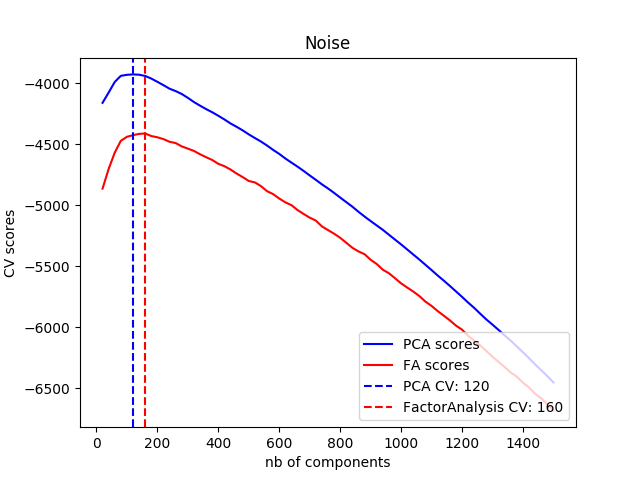
\includegraphics[width=1\textwidth]{images/pca_coarse.png}
  \end{minipage}
  \label{fig:pca_coarse}
  }
  \subfigure[Fine-Grained]{
  \begin{minipage}[t]{0.225\textwidth}
      \centering
      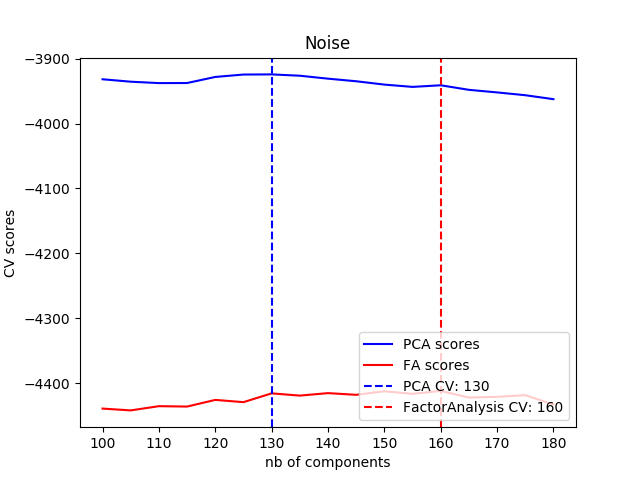
\includegraphics[width=1\textwidth]{images/pca_fine.png}
  \end{minipage}
  \label{fig:pca_fine}
  }
\caption{PCA}
\label{fig:pca}
\end{figure}

\begin{table}[!b]
  \centering
  \caption{The Prediction Results with Dataset Augmentation} 
  \label{tab:ridge_aug}
  \begin{tabular}{c|c}
  \toprule
  Dataset & Private Leaderboard Accuracy\\
  \midrule
  Original & 0.92994 \\
  Augmentation Iter 1 & 0.93708 \\
  Augmentation Iter 2 & 0.93727 \\
  Augmentation Iter 3 & 0.93754 \\
  \bottomrule
  \end{tabular}
\end{table}

\begin{figure*}[!t]
  \centering
  \subfigure[Pre=L1]{
  \begin{minipage}[t]{0.33\textwidth}
      \centering
      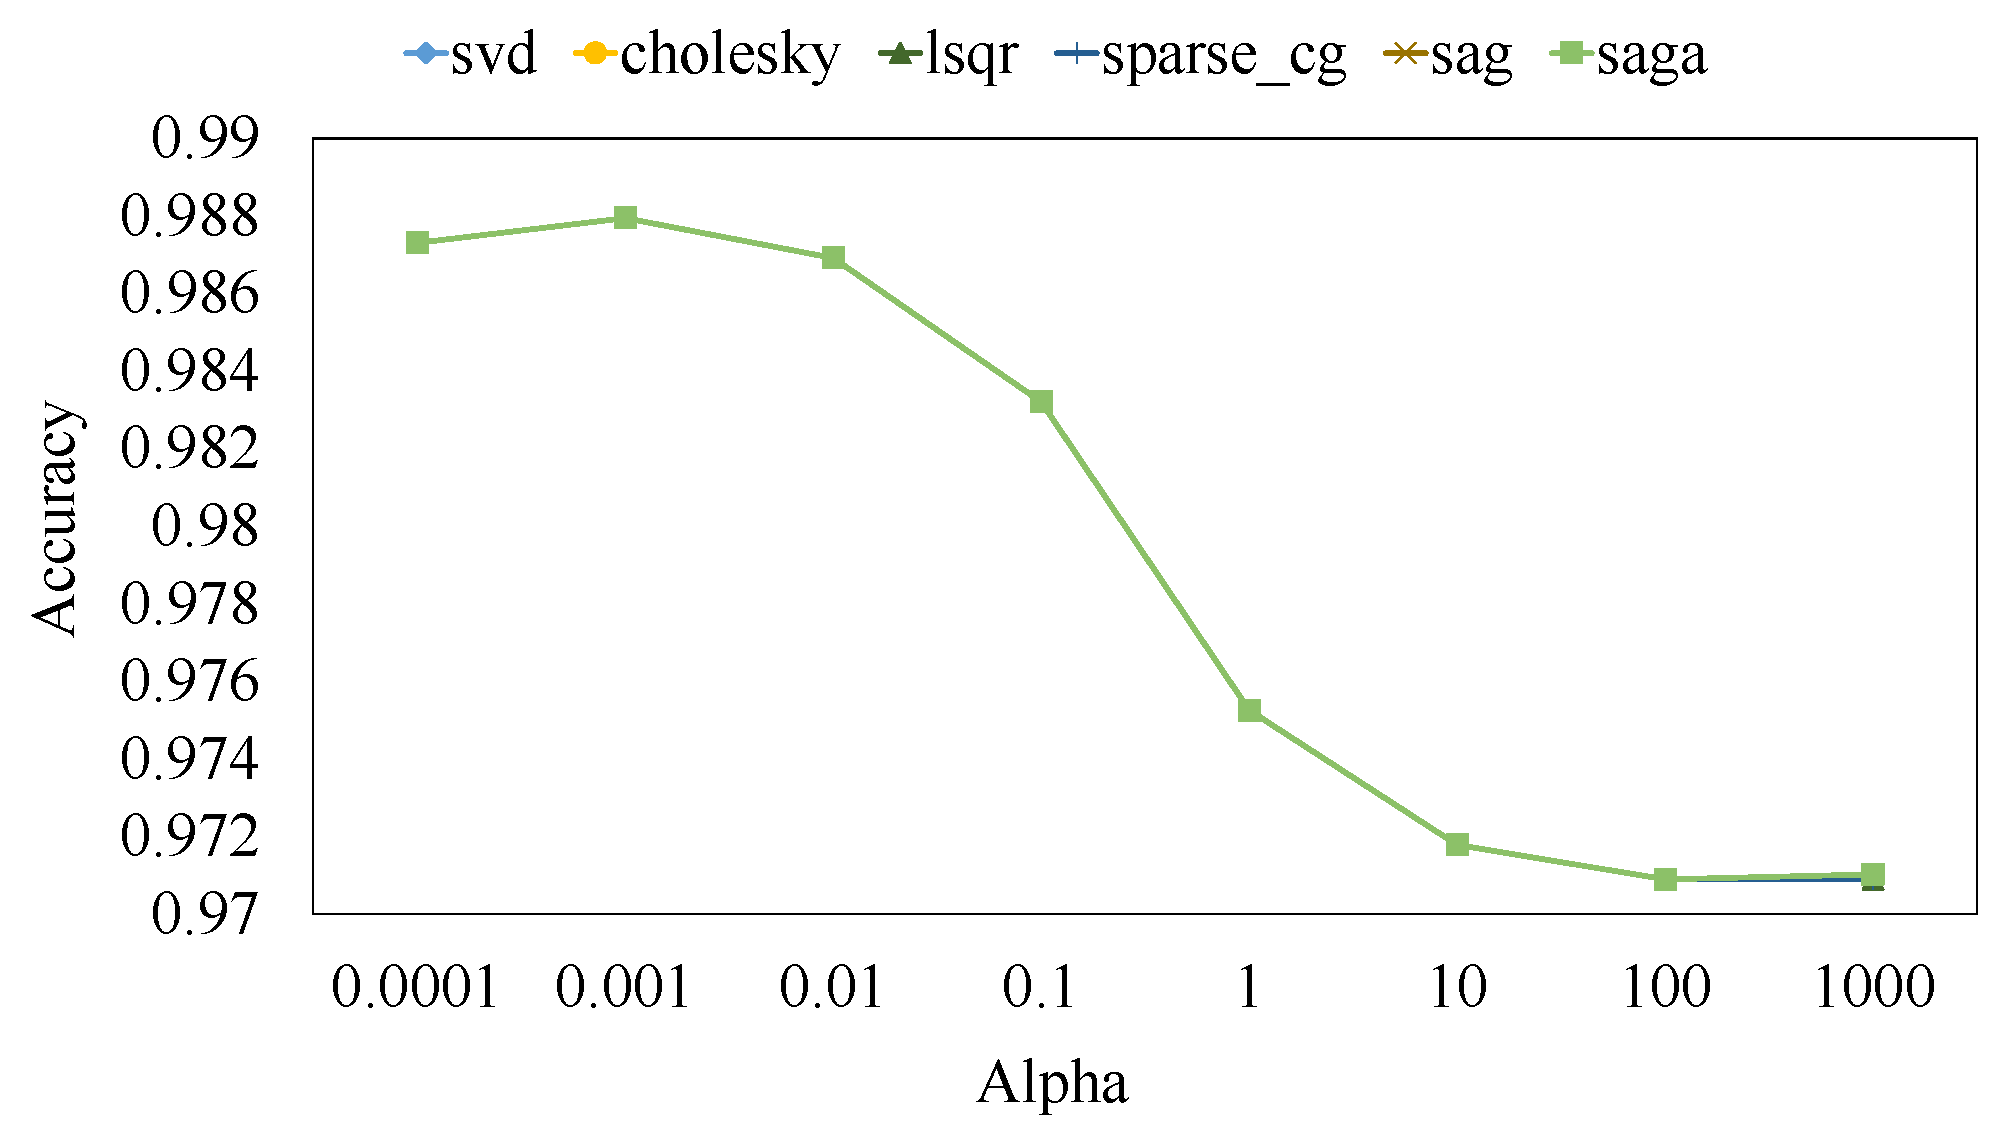
\includegraphics[width=1\textwidth]{images/ridgel1}
  \end{minipage}
  \label{fig:ridge_l1}
  }%
  \subfigure[Pre=L2]{
  \begin{minipage}[t]{0.33\textwidth}
      \centering
      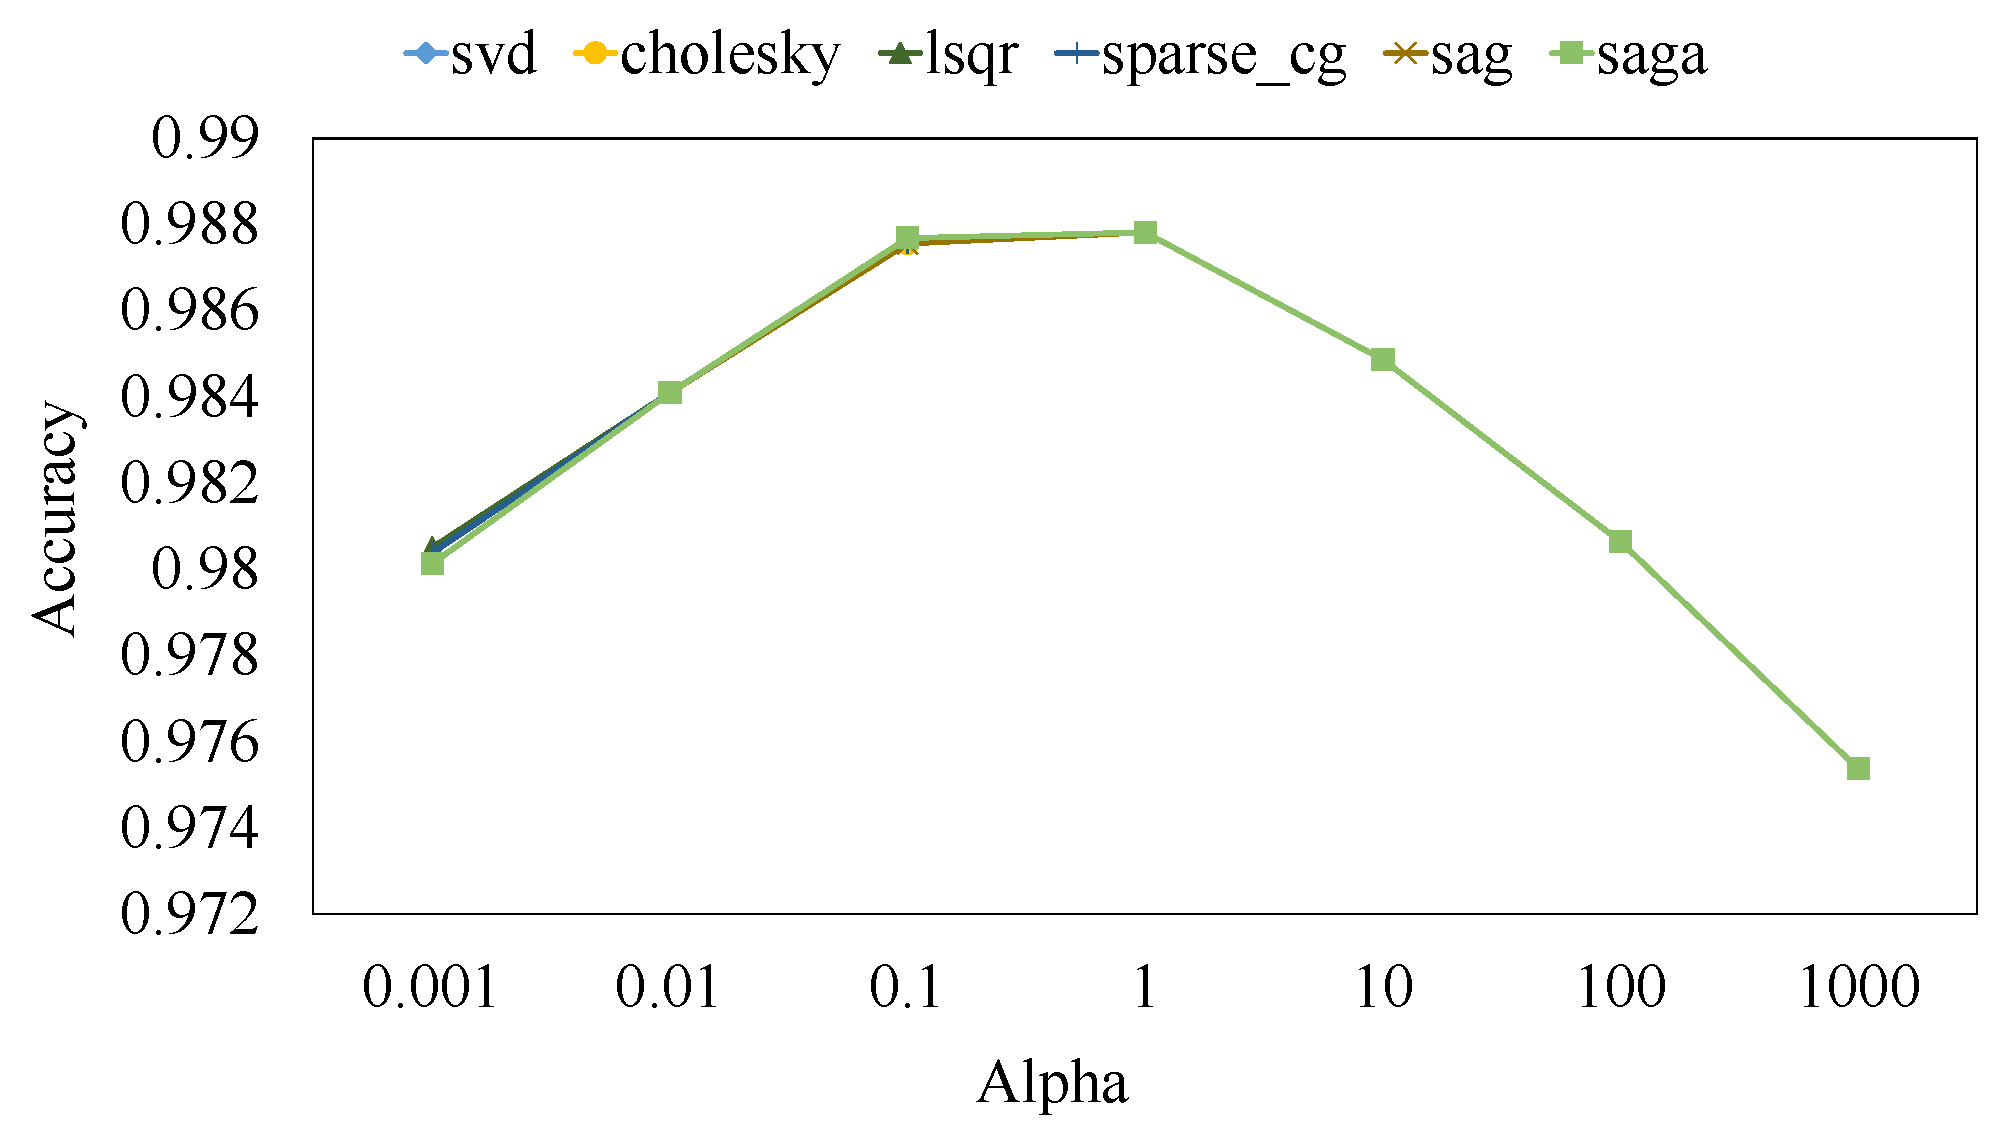
\includegraphics[width=1\textwidth]{images/ridgel2}
  \end{minipage}
  \label{fig:ridge_l2}
  }%
  \subfigure[Pre=Min-Max]{
  \begin{minipage}[t]{0.33\textwidth}
      \centering
      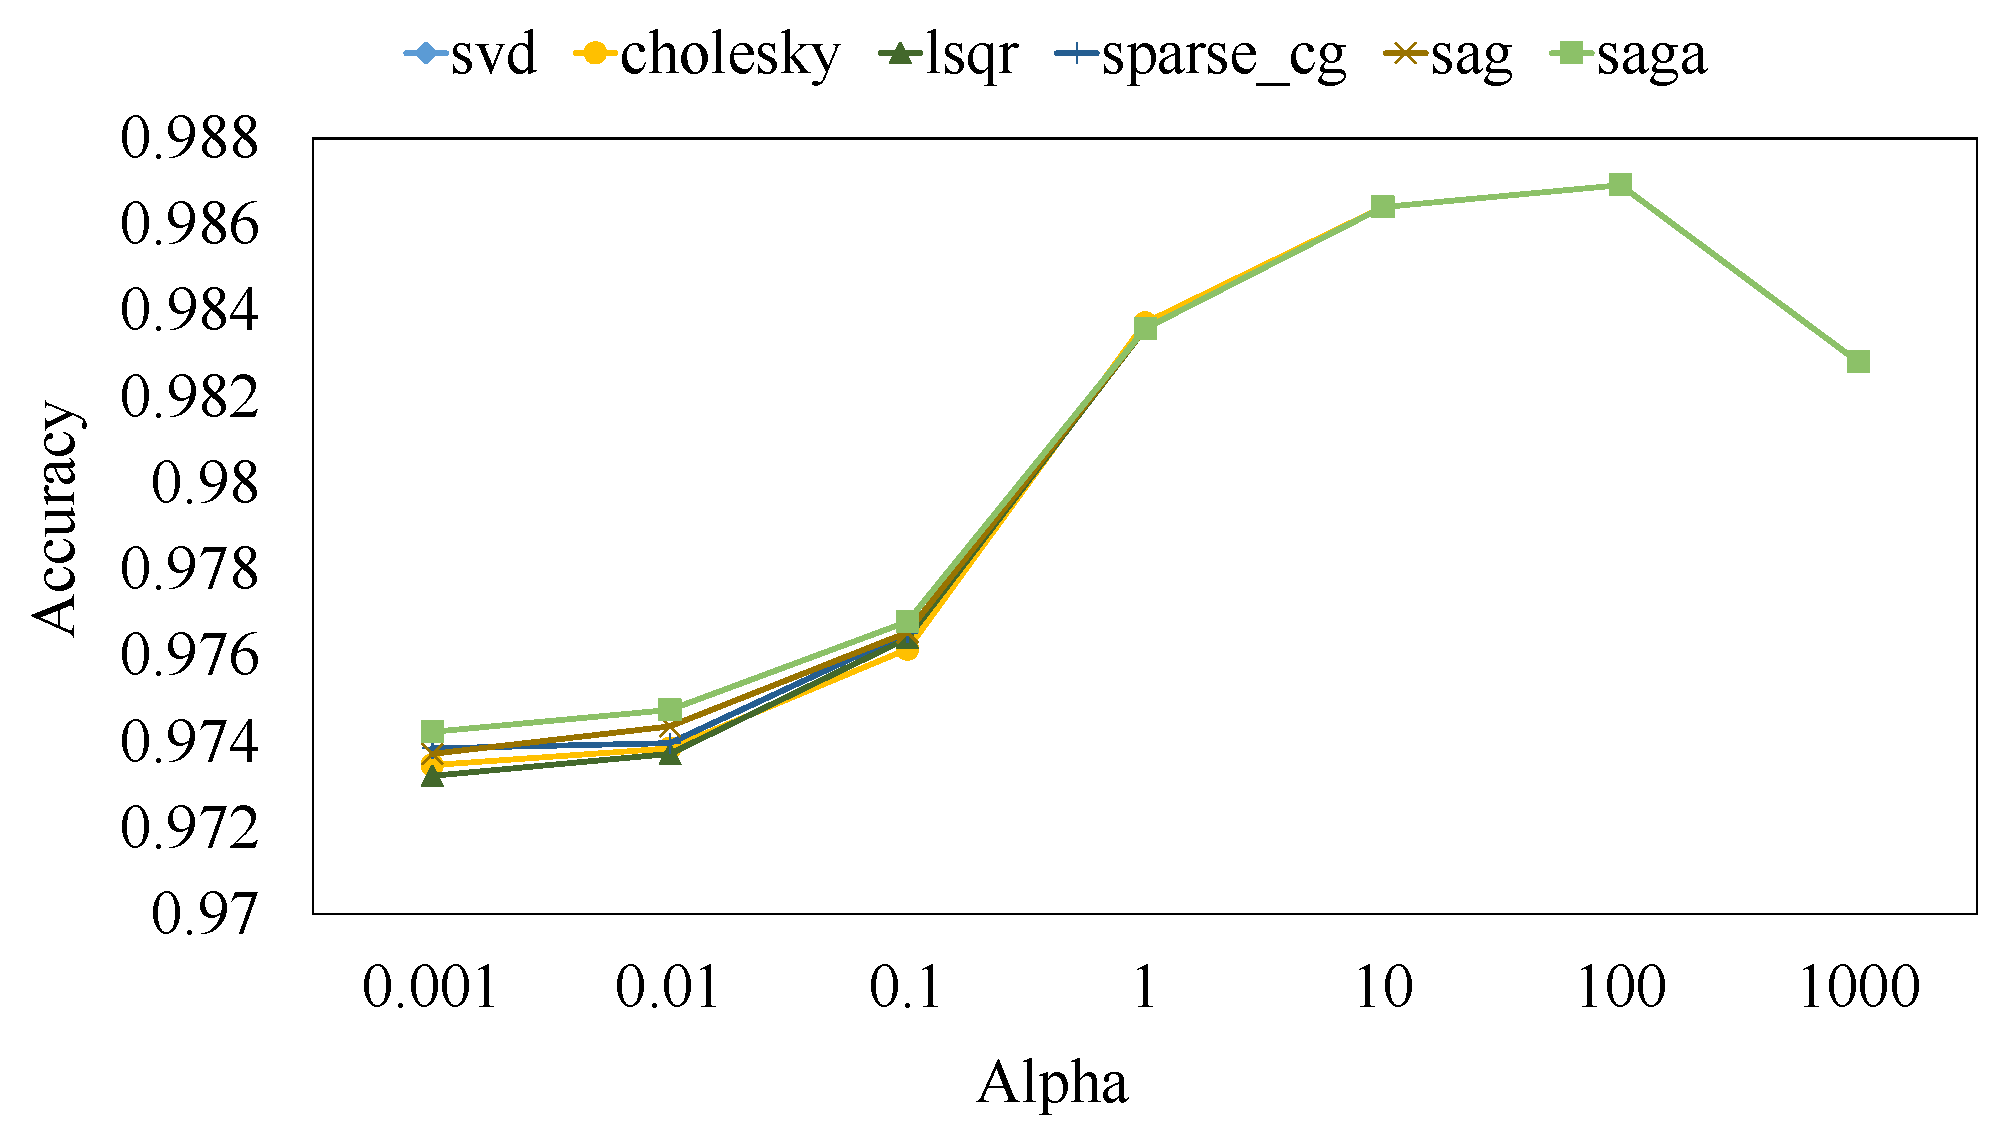
\includegraphics[width=1\textwidth]{images/ridgeminmax}
  \end{minipage}
  \label{fig:ridge_minmax}
  }
\caption{Ridge Classification}
\label{fig:ridge}
\end{figure*}

\section{Evaluation}
\label{sec:evaluation}
In this section, we present our evaluation of all of the above methods, and the accuracy in the evaluation is based on the 5-fold cross-validation on the training set unless otherwise stated.

\subsection{Dataset Augmentation}
\label{subsec:dataset_aug}
As we mentioned in \ref{subsec:augmentation}, our best model is obtained by training on the augmented dataset. In practice, we combined the prediction results of ridge classification, logistic regression and linear discriminant analysis these three classifiers. As this process is repeated, the results are shown in Table \ref{tab:ridge_aug}.

\subsection{PCA}
\label{subsec:eva_pca}
As we have mentioned in \ref{subsec:fa}, following the instructions given in \cite{pcavsfa}, we draw the results as shown in Figure \ref{fig:pca}. In Figure \ref{fig:pca_coarse}, we set the dimension range from 20 to 1500 with a span of 20. In Figure \ref{fig:pca_fine}, we set the dimension range from 100 to 180 with a span of 5.

\subsection{Ridge Classification}
\label{subsec:eva_ridge}
In this subsection, we compare the prediction accuracy under different solvers by setting different alpha values under different preprocessing. The experiment results are drawn in Figure \ref{fig:ridge}. Basically, different solvers have little effect on prediction accuracy. In Figure \ref{fig:ridge_l1}, we performed l1 normalization on the data and the prediction accuracy reaches a maximum of 0.98795 at alpha=0.001. In Figure \ref{fig:ridge_l1}, we performed l2 normalization on the data and the prediction accuracy reaches a maximum of 0.98782 at alpha=1. In Figure \ref{fig:ridge_minmax}, we performed min-max scaling on the data and the prediction accuracy reaches a maximum of 0.98692 at alpha=100.

\subsection{Logistic Regression}
\label{subsec:eva_logreg}

Fix the value of the parameter 'multi\_class' as 'ovr', we compare the performance under different solvers by setting different C under different penalty. The experiment results are drawn in Figure \ref{fig:logreg}. Set the penalty as 'l1', with C equal to 0.1, both valid solvers saga and liblinear have achieved the highest prediction accuracy of 0.98385 and 0.9841, respectively. Set the penalty as 'l2', solver newton-cg and lbfgs reach the highest prediction accuracy of 0.98513 at C=0.01.

\begin{figure}[!t]
  \centering
  \subfigure[Penalty=L1]{
  \begin{minipage}[t]{0.225\textwidth}
      \centering
      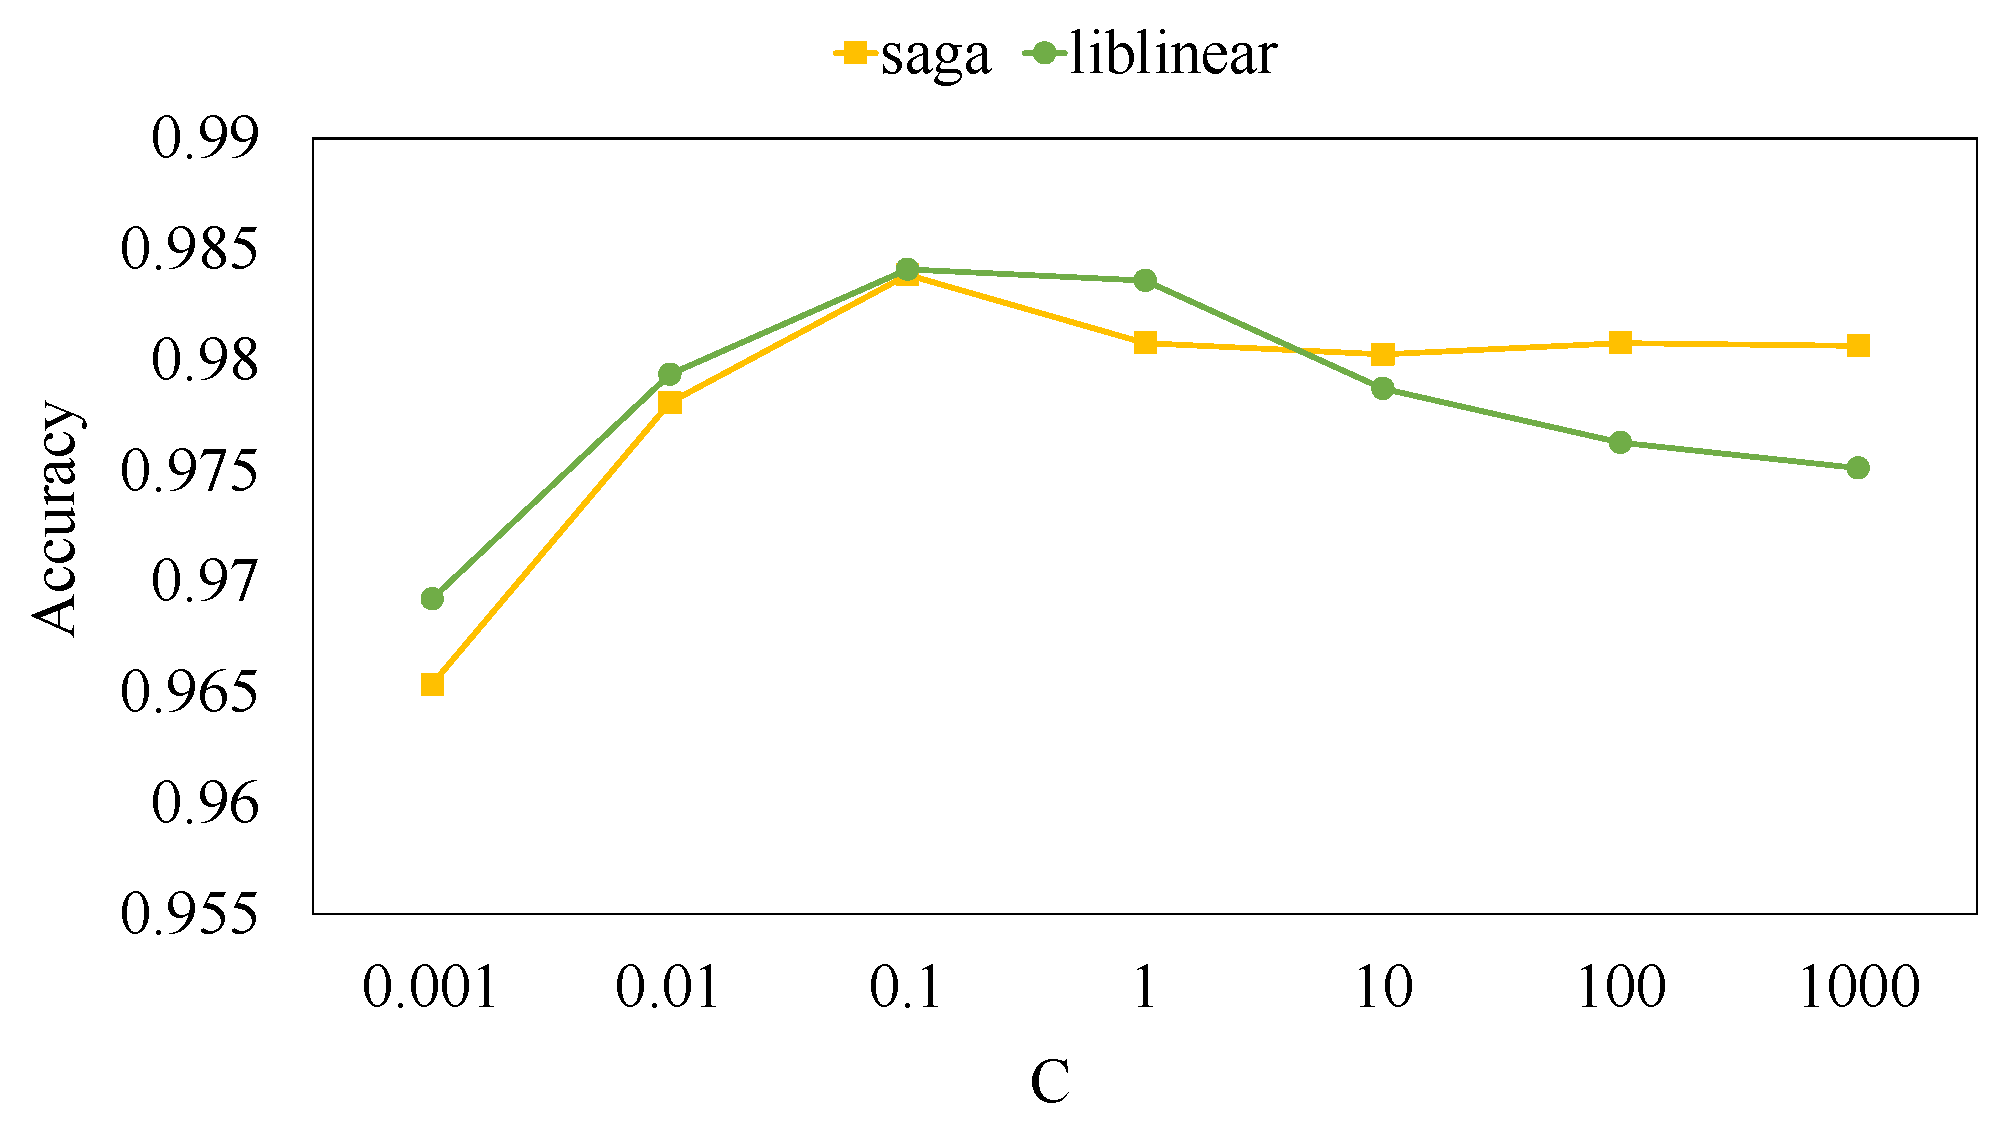
\includegraphics[width=1\textwidth]{images/logregl1}
  \end{minipage}
  \label{fig:logreg_l1}
  }
  \subfigure[Penalty=L2]{
  \begin{minipage}[t]{0.225\textwidth}
      \centering
      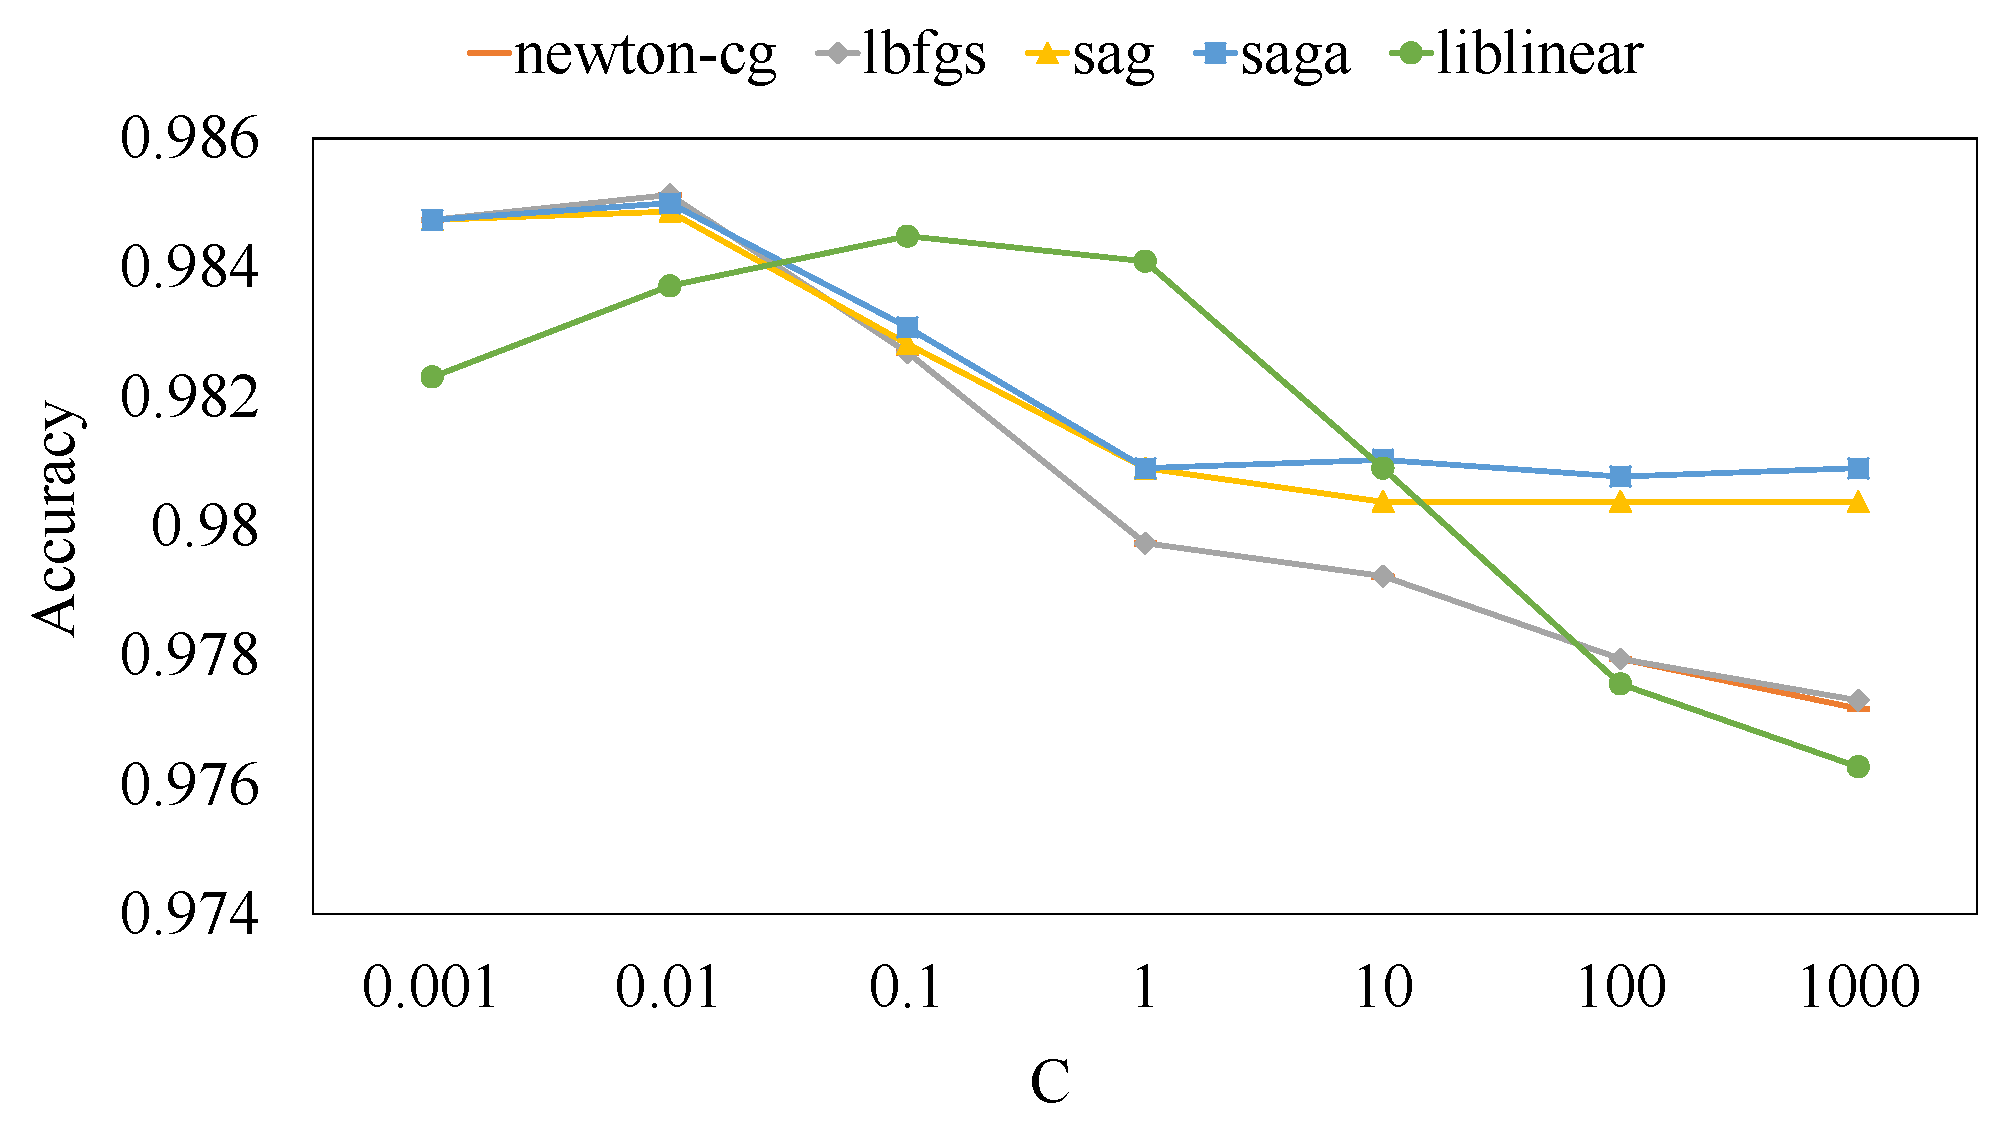
\includegraphics[width=1\textwidth]{images/logregl2}
  \end{minipage}
  \label{fig:logreg_l2}
  }
\caption{Logistic Regression}
\label{fig:logreg}
\end{figure}

\subsection{LDA}
\label{subsec:eva_lda}
When using LDA without performing dimensionality reduction of the original data first, the program will give a warning that variables are collinear and the prediction accuracy is low. So, in this subsection, using PCA to reduce the original data to different dimensions, we show the performance of LDA with different solvers in Figure \ref{fig:lda}. When the dimension of the data is not reduced, the prediction accuracy of LDA is only 0.97346, which is lower than the accuracy when the data is reduced to 50 dimensions in the figure.

\subsection{SVM}
\label{subsec:eva_svm}
Figure \ref{fig:svm} shows the prediction accuracy of linear svc under different C when l1 and l2 are used as penalty separately. With penalty as l1, it achieves highest prediction accuracy 0.9841 when C equals to 0.01. Similarly, with penalty as l2, the highest prediction accuracy is 0.98474 when C equals to 0.01.

\begin{figure}[!t]
  \centering
  \begin{minipage}[t]{0.225\textwidth}
    \centering
    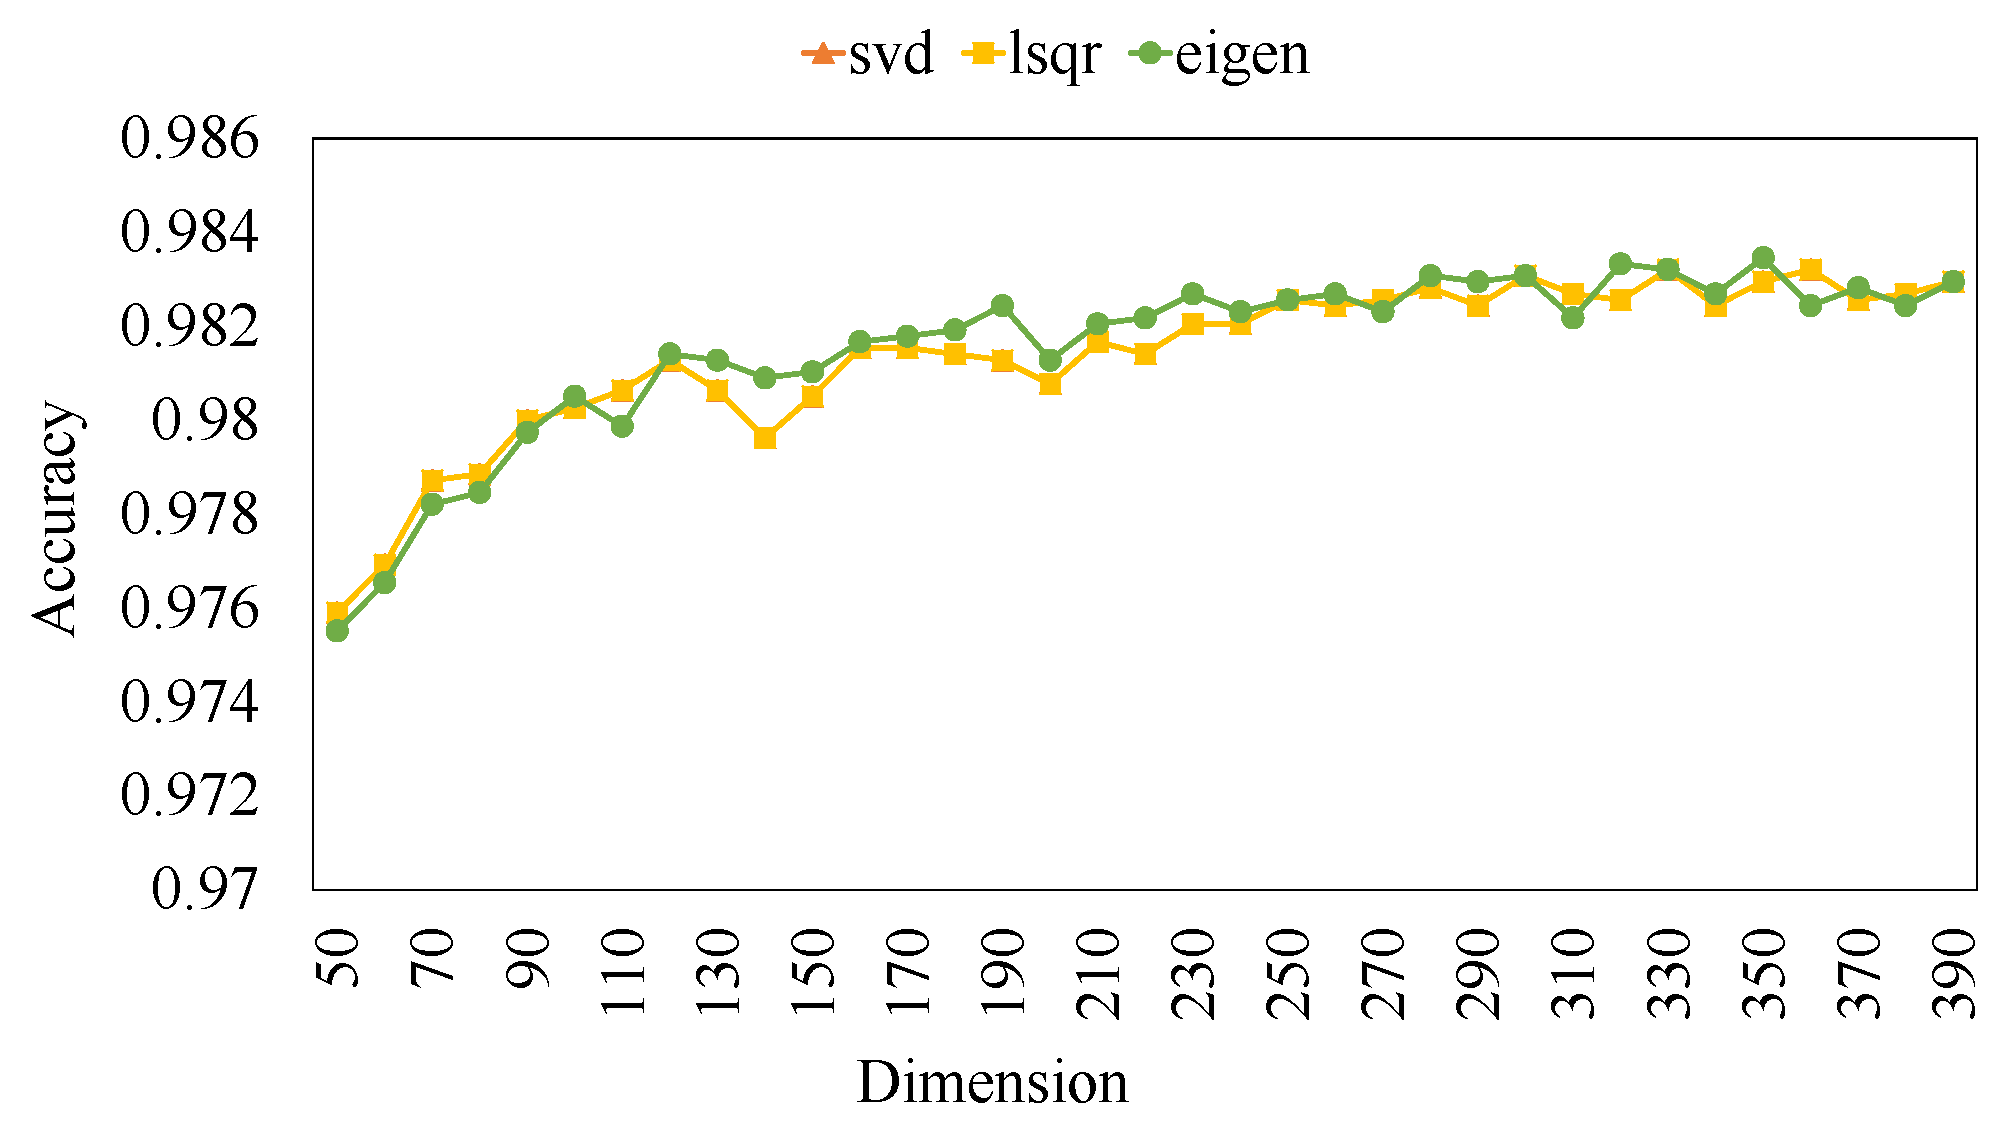
\includegraphics[width=1\textwidth]{images/lda}
    \caption{LDA}
    \label{fig:lda}
  \end{minipage}
  \begin{minipage}[t]{0.225\textwidth}
    \centering
    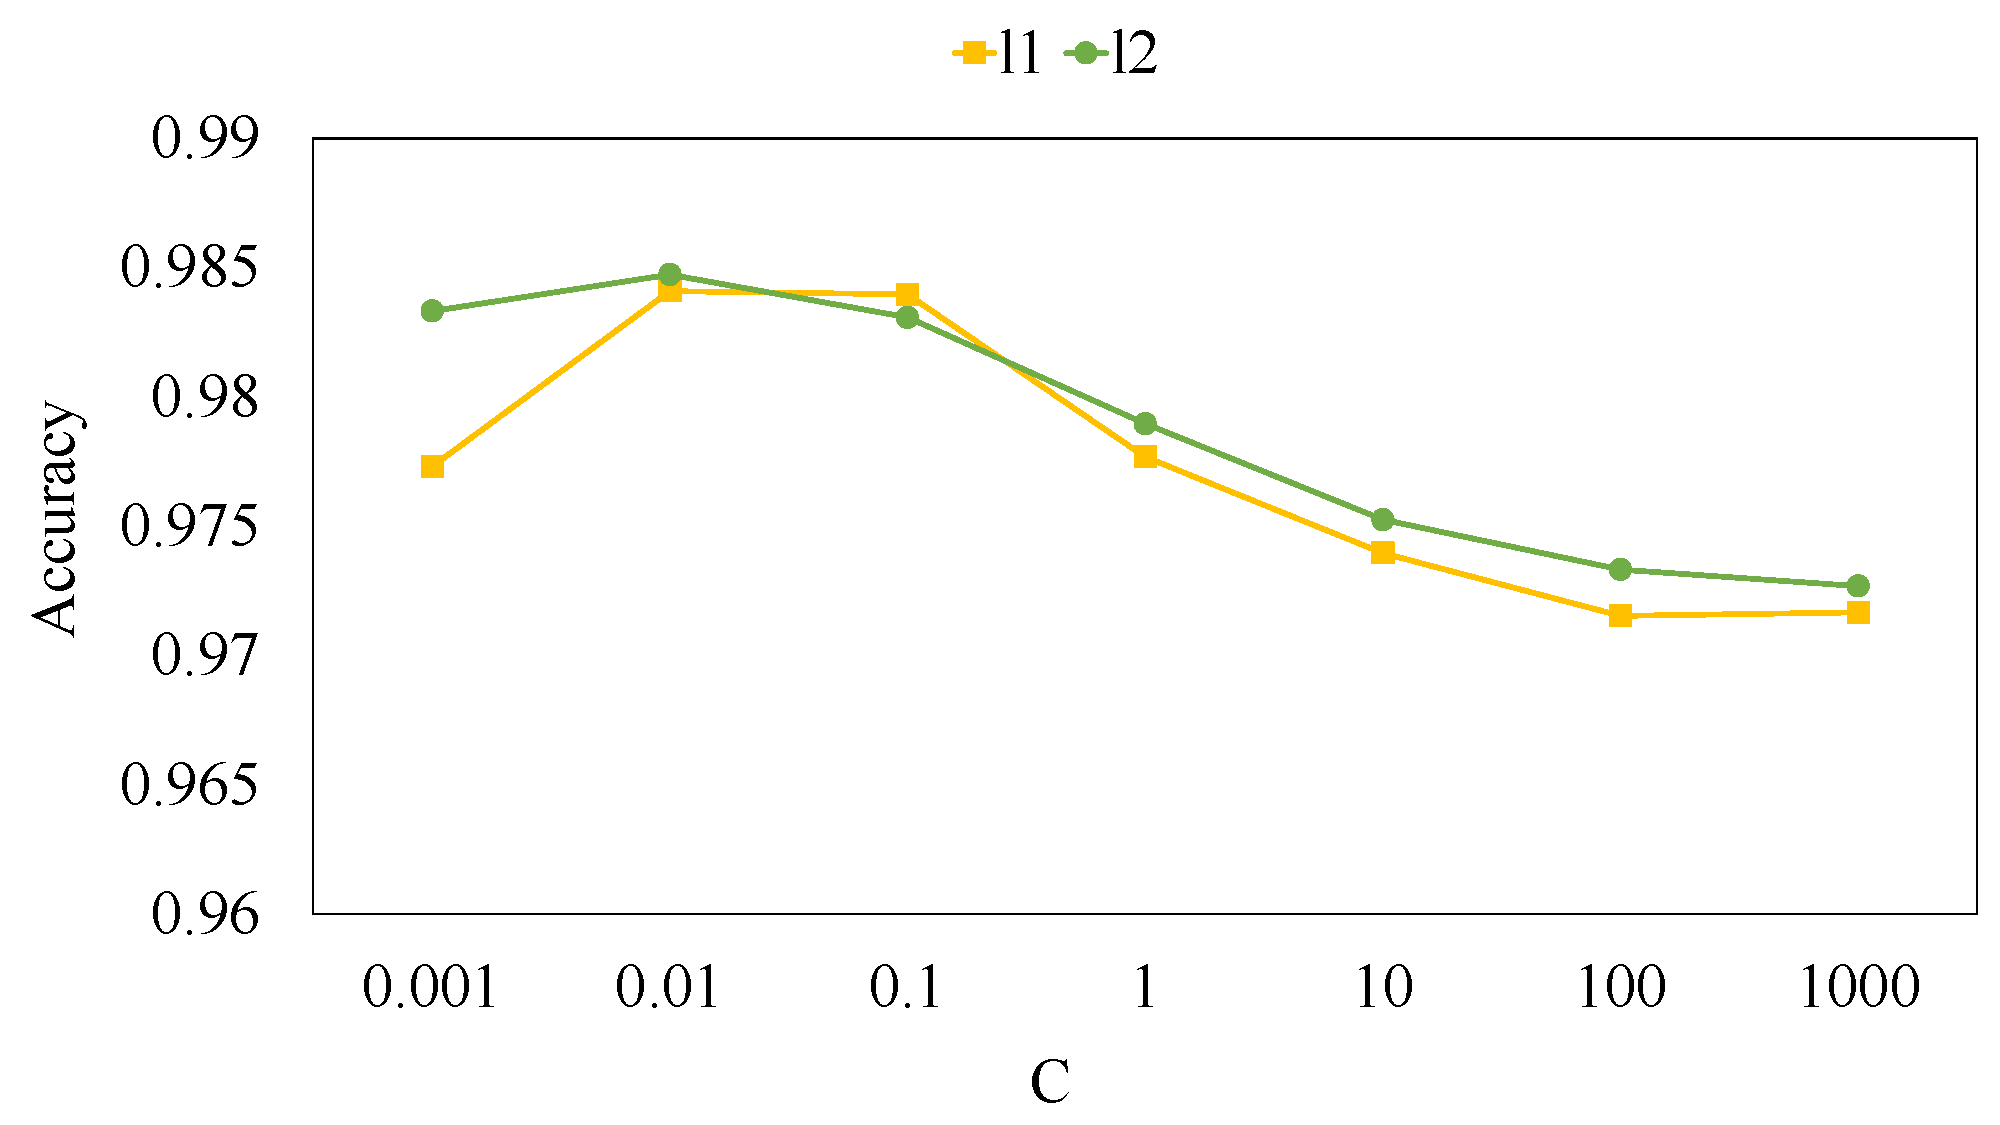
\includegraphics[width=1\textwidth]{images/linsvm}
    \caption{SVM}
    \label{fig:svm}
  \end{minipage}
\end{figure}

\subsection{KNN}
\label{subsec:eva_knn}
Setting the power parameter of Minkowski metric to 1 and 2, respectively, we plot the prediction accuracy under different K values with weights set to uniform and distance in Figure \ref{fig:knn}. For power equals to 2, when we choose distance mode as weight function, the estimator reaches the highest prediction accuracy of 0.97385 at K=7. For power equals to 1, the estimator reaches the highest prediction accuracy of 0.97462 at K=18.

\begin{figure}[!t]
  \centering
  \subfigure[Power=1]{
  \begin{minipage}[t]{0.225\textwidth}
      \centering
      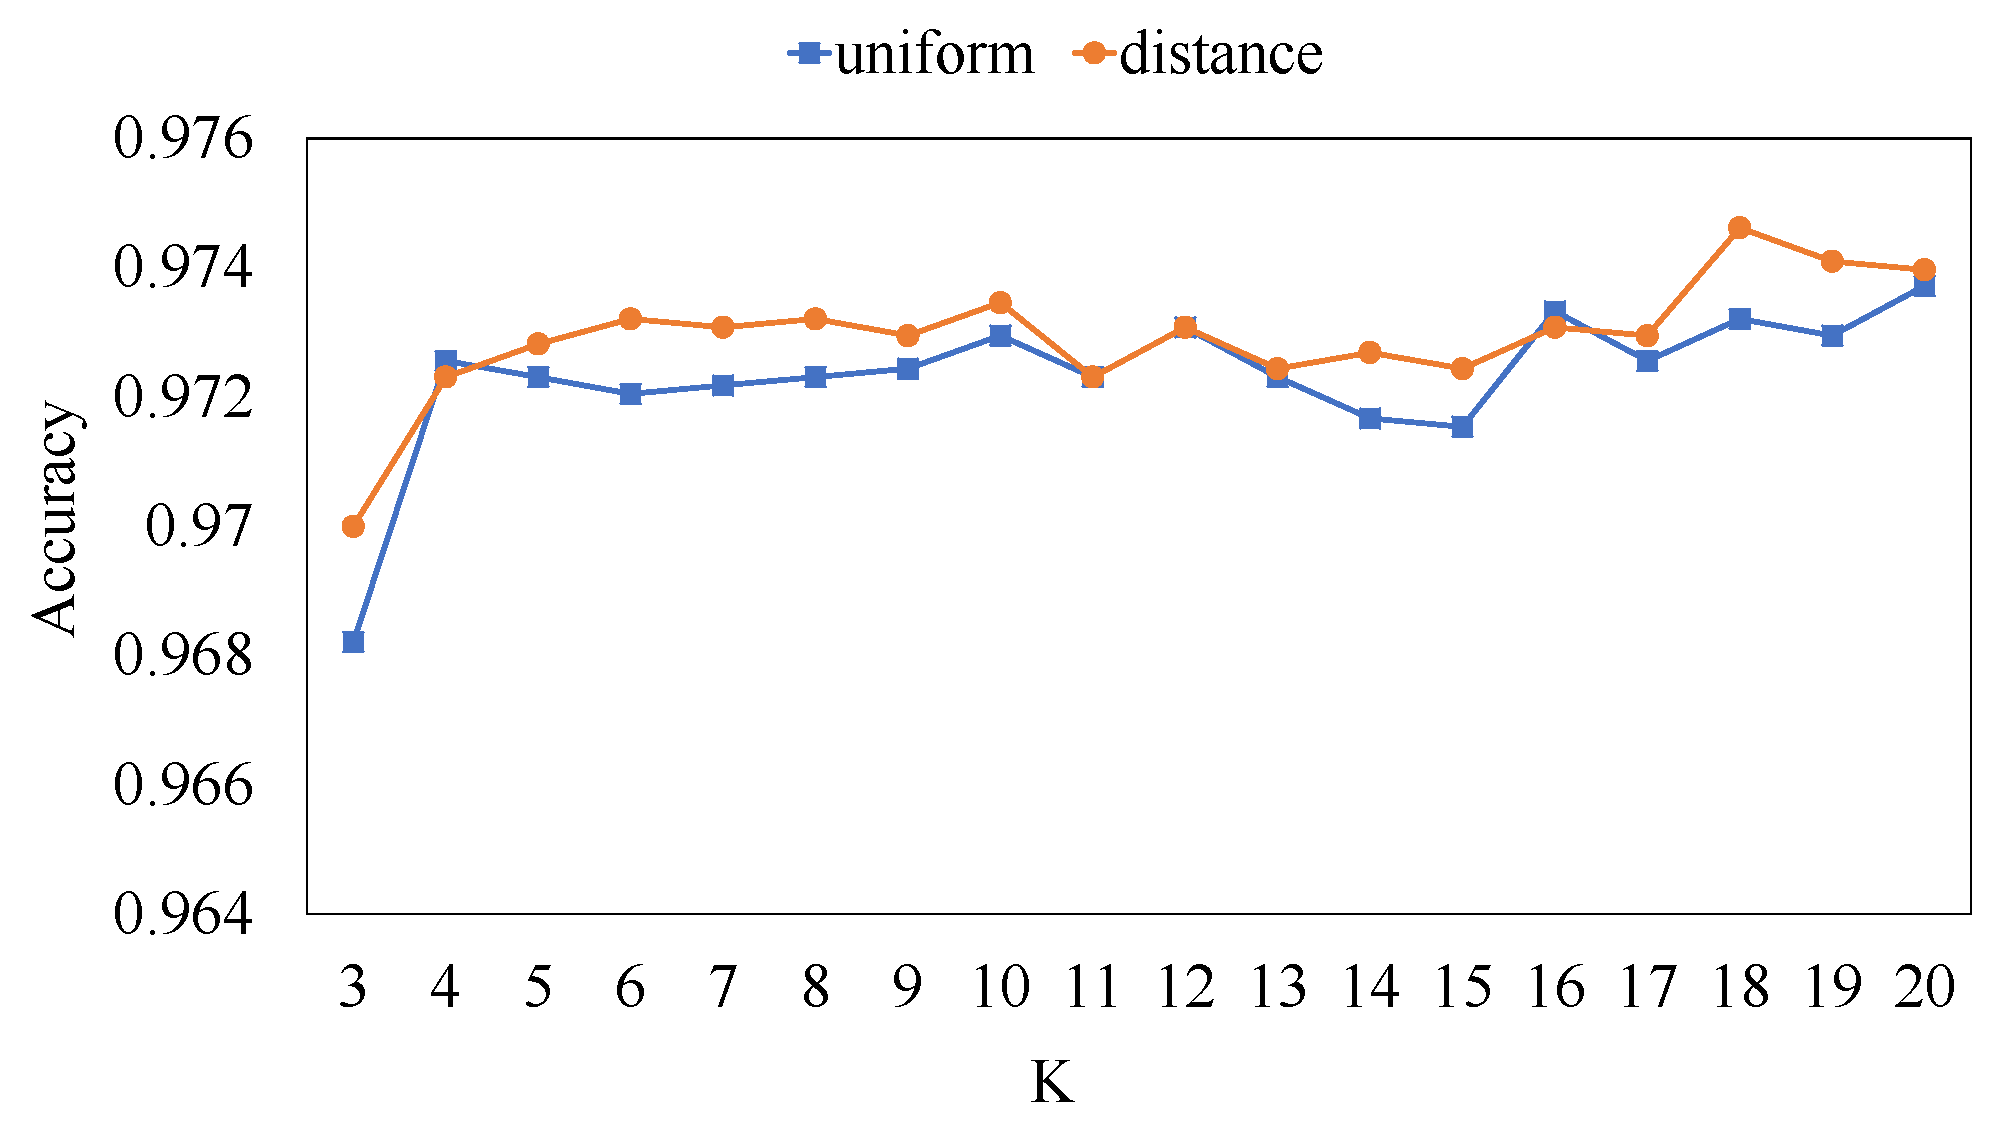
\includegraphics[width=1\textwidth]{images/knnp1}
  \end{minipage}
  \label{fig:knn_p1}
  }
  \subfigure[Power=2]{
  \begin{minipage}[t]{0.225\textwidth}
      \centering
      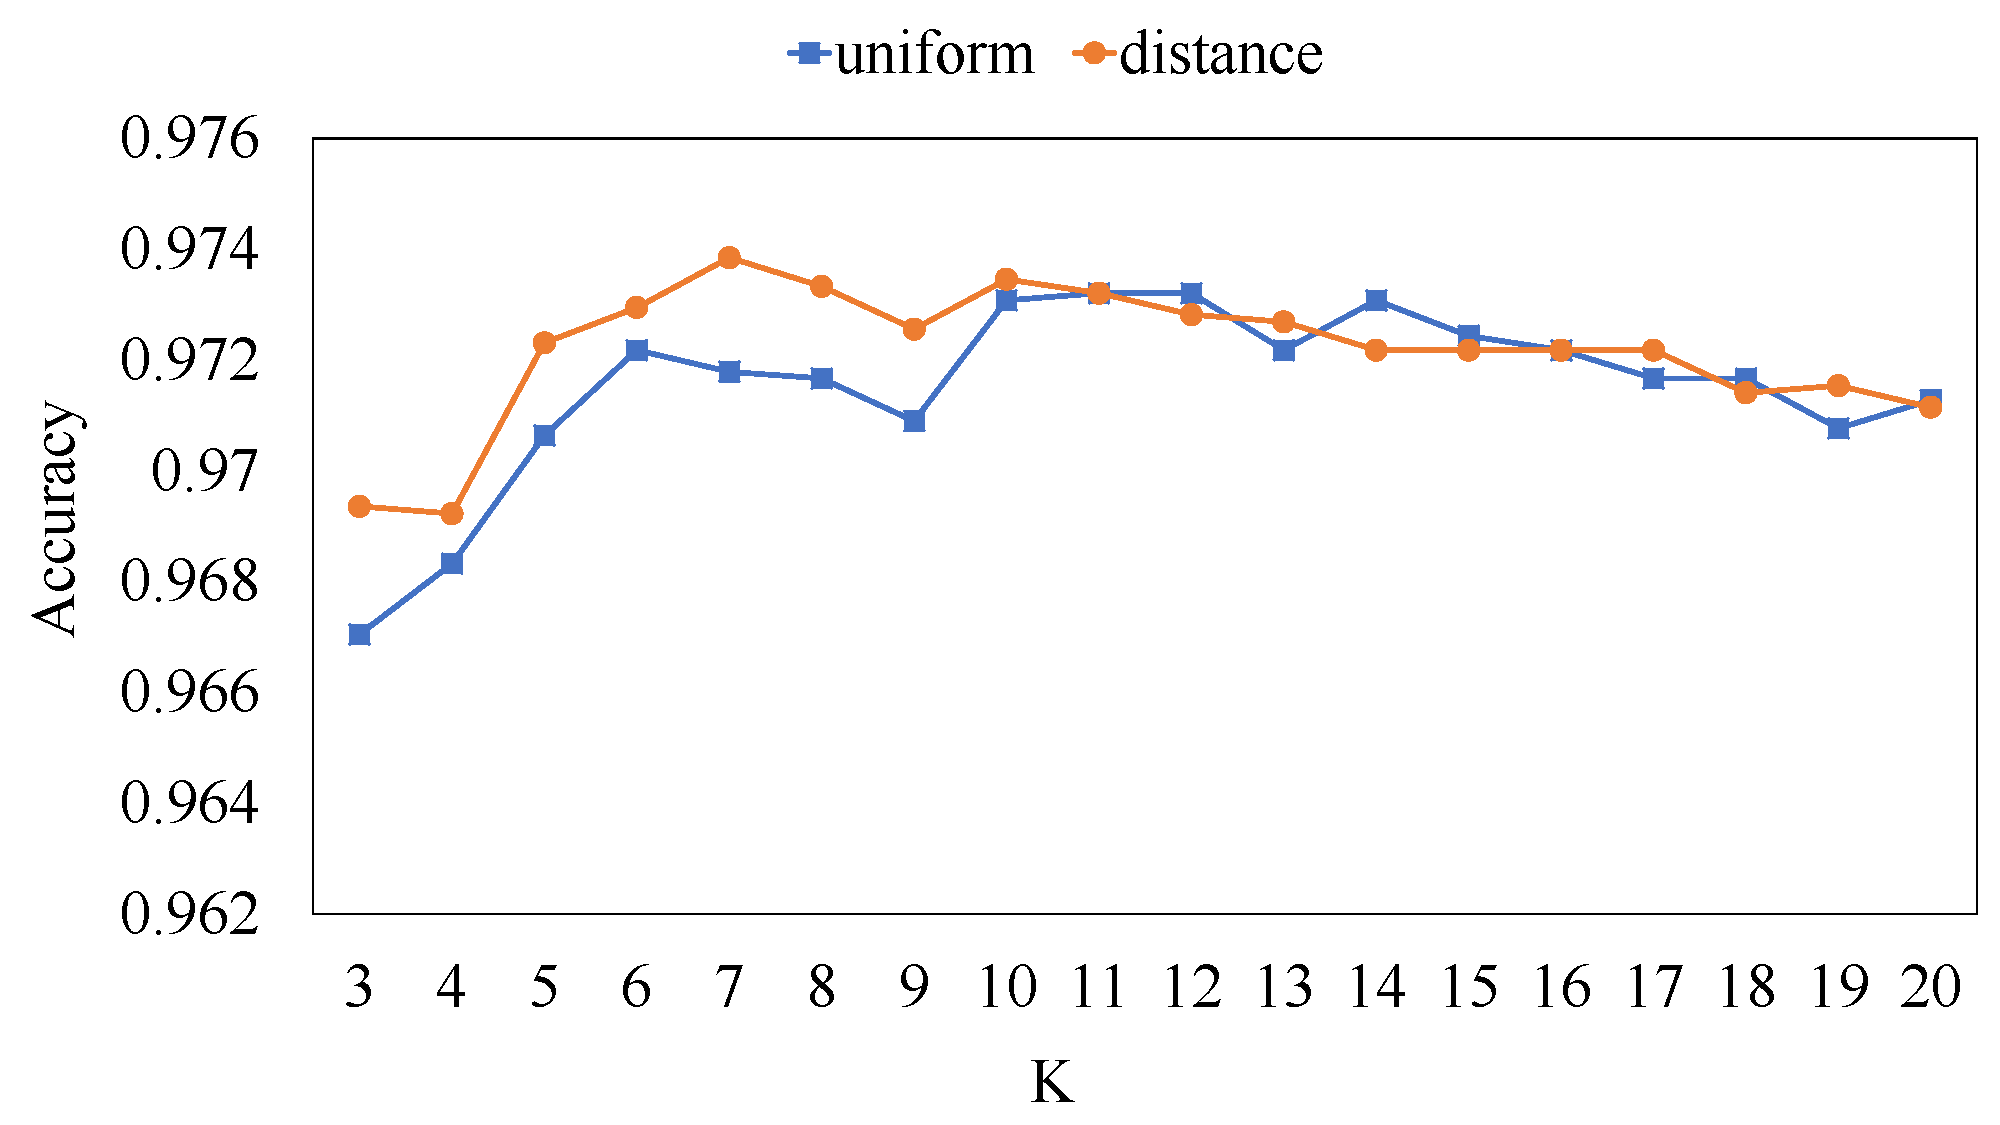
\includegraphics[width=1\textwidth]{images/knnp2}
  \end{minipage}
  \label{fig:knn_p2}
  }
\caption{KNN}
\label{fig:knn}
\end{figure}

\section{Conclusion}
\label{sec:conclusion}

In this paper, we have used ridge classification, logistic regression, linear discriminant analysis, support vector machine and k nearest neighbour classification these five approaches to perform image classification. We have also tried data preprocessing and dimensionality reduction. When we hit the accuracy wall, we propose to use the semi-supervised learning method to augment the dataset to further improve the prediction accuracy of the model. And finally we achieved an accuracy of 0.93754 on the test set and ranked 37th on the private leaderboard.


% use section* for acknowledgment
\ifCLASSOPTIONcompsoc
  % The Computer Society usually uses the plural form
  \section*{Acknowledgments}
\else
  % regular IEEE prefers the singular form
  \section*{Acknowledgment}
\fi


The author would like to thank Prof. Liqing Zhang and TA Jianfu Zhang and Xiang Li for their instructions on this work.


% Can use something like this to put references on a page
% by themselves when using endfloat and the captionsoff option.
\ifCLASSOPTIONcaptionsoff
  \newpage
\fi



% trigger a \newpage just before the given reference
% number - used to balance the columns on the last page
% adjust value as needed - may need to be readjusted if
% the document is modified later
%\IEEEtriggeratref{8}
% The "triggered" command can be changed if desired:
%\IEEEtriggercmd{\enlargethispage{-5in}}

% references section

% can use a bibliography generated by BibTeX as a .bbl file
% BibTeX documentation can be easily obtained at:
% http://mirror.ctan.org/biblio/bibtex/contrib/doc/
% The IEEEtran BibTeX style support page is at:
% http://www.michaelshell.org/tex/ieeetran/bibtex/
%\bibliographystyle{IEEEtran}
% argument is your BibTeX string definitions and bibliography database(s)
%\bibliography{IEEEabrv,../bib/paper}
%
% <OR> manually copy in the resultant .bbl file
% set second argument of \begin to the number of references
% (used to reserve space for the reference number labels box)
\iffalse
\begin{thebibliography}{1}

\bibitem{IEEEhowto:kopka}
H.~Kopka and P.~W. Daly, \emph{A Guide to \LaTeX}, 3rd~ed.\hskip 1em plus
  0.5em minus 0.4em\relax Harlow, England: Addison-Wesley, 1999.

\end{thebibliography}
\fi

\bibliographystyle{IEEEtran}
\bibliography{ref}

% biography section
% 
% If you have an EPS/PDF photo (graphicx package needed) extra braces are
% needed around the contents of the optional argument to biography to prevent
% the LaTeX parser from getting confused when it sees the complicated
% \includegraphics command within an optional argument. (You could create
% your own custom macro containing the \includegraphics command to make things
% simpler here.)
%\begin{IEEEbiography}[{\includegraphics[width=1in,height=1.25in,clip,keepaspectratio]{mshell}}]{Michael Shell}
% or if you just want to reserve a space for a photo:


% You can push biographies down or up by placing
% a \vfill before or after them. The appropriate
% use of \vfill depends on what kind of text is
% on the last page and whether or not the columns
% are being equalized.

%\vfill

% Can be used to pull up biographies so that the bottom of the last one
% is flush with the other column.
%\enlargethispage{-5in}



% that's all folks
\end{document}


